\documentclass{beamer}
\mode<presentation>
%\usetheme{Warsaw}
\usetheme{Warsaw}
\setbeamertemplate{headline}{}
\usecolortheme{dolphin}
\setbeamerfont{frametitle}{size=\bfseries,series=\bfseries,parent=structure}
    \setbeamerfont{title}{series=\bfseries,parent=structure}
    \setbeamerfont{subtitle}{size=\scriptsize,series=\bfseries,parent=structure}
    \setbeamerfont{author}{size=\scriptsize,series=\bfseries,parent=structure}
    \setbeamerfont{institute}{size=\scriptsize,series=\bfseries,parent=structure}
    \setbeamerfont{date}{size=\scriptsize,series=\bfseries,parent=structure}
\setbeamercovered{transparent}
\setbeamerfont{page number in head/foot}{size=\large}
\setbeamertemplate{footline}[frame number]
%\setbeamertemplate{caption}[numbered]
\usepackage{etoolbox}
\makeatletter
\patchcmd{\beamer@sectionintoc}{\vfill}{\vskip 1.5em}{}{} %\vskip1.5em \itemsep
\makeatother

 \usepackage[english]{babel}
 \usepackage[latin1]{inputenc}
\usepackage[T1]{fontenc}
\usepackage{helvet}
\usepackage{slashed}
\usepackage{color}
\usepackage{xcolor}
\usepackage{multicol}
\usepackage{subfigure}
 \usepackage{movie15}
 \usepackage{animate}
\usepackage{hyperref}
\usepackage{subfigure}
\usefonttheme[onlymath]{serif}
%%% new commands and macros %%%%%%%%%%%%%%%%%%%%%%%%%%%%%%%%%%%%%%%%%%%
\newlength{\figwidth}
\setlength{\figwidth}{0.9\columnwidth}

\newlength{\qfigheight}
\setlength{\qfigheight}{0.25\textheight}

\newlength{\hfigheight}
\setlength{\hfigheight}{0.5\textheight}

\newcommand{\dedicationfont}{\fontencoding{T1}\fontfamily{anttlc}\fontseries{m}\fontshape{n}\fontsize{12}{15}\selectfont}

\newcommand{\acro}[1]{#1\@}
\newcommand{\abbr}[1]{\textsc{\texttt{#1}}}
\newcommand{\abbrlc}[2]{\textsc{\texttt{#1}}\texttt{#2}}
\newcommand{\desg}[1]{\texttt{#1}}
\newcommand{\todo}[1]{\textbf{\uppercase{\emph{#1}}}} %\textcolor{Orange}{#1}}}


%Some variables
%
%
\def\g12{\emph{g12}}

\def\G11{\emph{g11}}
\def\clas{\abbr{CLAS }}

\def\Lqcd{\mathcal{L}_{\mathtt{QCD}}}
\def\qfield{\psi}
\def\qbarfield{\overline{\psi}}

\def\grpath{/Users/Mike/phdthesis/MY_THESIS/figures/print}
\def\figures{/Users/Mike/phdthesis/MY_THESIS/figures/print}

\newcommand{\bank}[4]{$\mathtt{#1}^{#2}_{#3}\lbrack\mathtt{#4}\rbrack$}

\def\ith{$i$\textsuperscript{th}}

\def\um{{\text{$\mu$}}m}

%\def\coloronline{(Color online.)\ }
\def\coloronline{}

%%% particles
\def\p{\mathrm{p}}
\def\n{\mathrm{n}}
\def\Kp{\mathrm{K}^{+}}
\def\Km{\mathrm{K}^{-}}
\def\K0{\mathrm{K}^{0}}
\def\Y{\mathrm{Y}}
\def\epos{\mathrm{e}^{+}}
\def\eneg{\mathrm{e}^{-}}
\def\gamstar{\mathrm{$\gamma$}^{*}}
\def\piup{$\pi$}
\def\gammaup{$\gamma$}
%%% TAGGER and RF related times
\def\trf{t_{\mathtt{RF}}}
\def\ttag{t_{\mathtt{TAG}}}
\def\ttagrf{t_{\mathtt{TAG,RF}}}
\def\tprop{t_\mathrm{prop}}
\def\ttrigoffset{t_{\mathrm{trigger-offset}}}

%%% BEAM energy
\def\ebeam{E_{\mathrm{beam}}}

%%% Beta
\def\betasttof{\beta_{\mathtt{ST-TOF}}}
\def\betatof{\beta_{\mathrm{vtx}\mathtt{-TOF}}}
\def\betap{\beta_{p}}

%%% path lengths
\def\lst{\ell_{\mathtt{ST}}}
\def\ltof{\ell_{\mathtt{TOF}}}
\def\lsttof{\ell_{\mathtt{ST-TOF}}}

%%% raw subsystem times
\def\tst{t_{\mathtt{ST}}}
\def\ttof{t_{\mathtt{TOF}}}
\def\dtsttof{\Delta t_{\mathrm{ST-TOF}}}

%%% vertex times
\def\tv{t_{\mathrm{vtx}}}
\def\tvtagrf{t_{\mathrm{vtx}}(\mathtt{TAG_{RF}})}
\def\tvst{t_{\mathrm{vtx}}(\mathtt{ST})}

\def\adcst{\mathtt{ADC}_{\mathtt{ST}}}

\newcommand{\bra}[1]{\left<#1\right|}
\newcommand{\ket}[1]{\left|#1\right>}
\newcommand{\braket}[2]{\left<#1\middle|#2\right>}
\def\piz{$\mathrm{\pi^{0}}\ $}
\def\epem{$e^+e^-\ $}
\title[Photoproduction of $\pi^0$ on $\ell$H$_2$ with \abbr{CLAS} from $\lowercase{e}^{+}\lowercase{e}^{-}\gamma$ decay]{Photoproduction of $\pi^0$ on hydrogen with CLAS from 1.1 GeV - 5.45 GeV from $\lowercase{e}^{+}\lowercase{e}^{-}\gamma$ decay}
%\title{Photoproduction of $\pi^0$ on hydrogen with CLAS from 1.1 GeV - 5.45 GeV from $\lowercase{e}^{+}\lowercase{e}^{-}\gamma$ decay}  
\subtitle{Michael C. Kunkel} %\\  Prof. Anatoly Radyushkin} 
\institute[ODU] % (optional, but mostly needed)
{
  %\inst{}%
 Old Dominion  University }

\date[October 15, 2014] % (optional)
{}

%\logo{\includegraphics[height=1cm]{odu.pdf}}
\begin{document}
\begin{frame}[plain]
  \titlepage
\end{frame}
% %
% %
\begin{frame}\frametitle{Outline}

\begin{multicols}{2}
%\tableofcontents  %[pausesections]


    \tableofcontents

\end{multicols}

  % You might wish to add the option [pausesections]
\end{frame}
\section{Introduction}
% %
\begin{frame}
\frametitle{Motivation} 
\begin{itemize}
\item We performed precise measurements of the \piz cross-section 
\begin{itemize}
\item Compare to existing data
\item Check validity of handbag model
\end{itemize}
\item Improve understanding of the \piz production in
\begin{itemize}
\item standard model applicable at lower energies 
\end{itemize}
\item New model appying the GPD handbag model applicable at higher energies 
\end{itemize}
\end{frame}
\section{\piz production}
\begin{frame}
\frametitle{\piz production}

\begin{figure}[h!]\begin{center}
\includegraphics[width=0.5 \figwidth,height=0.5 \qfigheight]{\figures/mike_defense_III.pdf}
\end{center}\end{figure}
\begin{itemize}
\item $\frac{d\sigma}{d\Omega} = \frac{q}{k}\left|\bra{\mathrm{\chi_{f}}}\cal{M} \ket{\mathrm{\chi_{i}}} \right|^2$ % 
\begin{itemize}
\item $\frac{d\sigma}{d\Omega} = \frac{1}{2} \frac{q}{k}\left(\left|H_N\right|^2 + \left|H_D\right|^2 + \left|H_{SP}\right|^2 + \left|H_{SA}\right|^2 \right)$ % 
\begin{itemize}
\item $H_N \equiv$ non-flip amplitudes
\item $H_D \equiv$ double-flip amplitudes
\item $H_{SP} \equiv$ single-flip amplitudes initial photon and nucleon having spins parallel
\item $H_{SA} \equiv$ single-flip amplitudes initial photon and nucleon having spins anti-parallel
\end{itemize}
\item Amplitudes have different kinematic dependence
\item Amplitudes are common to different reactions i.e. $\gamma p \to n \pi^+$, $\gamma p \to p \pi^0$, $\gamma n \to n \pi^-$
\end{itemize}
\item Model valid below 2.8~GeV currently
\end{itemize}
\end{frame}
\begin{frame}
\frametitle{\piz Production above 2.8~GeV} 
\begin{itemize}
\item \piz production is factorized into two parts
\begin{itemize}
\item one quark from the incoming and one from the outgoing nucleon participate in the hard sub-process (small blob)
\begin{itemize}
\item calculable using \abbr{pQCD}
\end{itemize}
\item The soft part consists of all the other partons that are spectators and can be described in terms of GPDs (large blob)
\end{itemize}
\end{itemize}
\begin{figure}[h!]\begin{center}
\includegraphics[width= \figwidth ,height=0.75 \hfigheight]{\figures/intro/handbag.pdf}

{\label{fig:xsection.handbag}	The handbag-type diagram for photoproduction of mesons.}
\end{center}\end{figure}
\end{frame}
\begin{frame}
\frametitle{\piz Production above 2.8~GeV} 
\begin{itemize}
\item Recent framework of handbag model led to \piz cross-section predictions
\end{itemize}
\begin{figure}[h!]\begin{center}
\includegraphics[width=\figwidth ,height=\hfigheight]{\figures/intro/photo-fig7.pdf}

{\label{fig:xsection.handbag.cal}The soft physics contribution to the cross-section for photoproduction of \piz scaled by s$^7$ versus $\cos\theta$, where $\theta$ is the scattering angle in the $\gamma p$ c.m. system and s is the total invariant energy squared.}
\end{center}\end{figure}

\end{frame}
\section{\piz decay}
\begin{frame}\frametitle{\piz Decay Modes} 
\begin{figure}[h!]\begin{center}
\subfigure[Feynman Diagram of \piz Two Photon Decay][]{ %Feynman diagram of \piz two photon decay
\includegraphics[width=0.75\figwidth,height=0.35\hfigheight]{\figures/intro/decays/P_to_gamgam_wnotation.pdf}\label{fig:piz.gamgam}}
\subfigure[Feynman Diagram of \piz Dalitz Decay][]{ %Feynman diagram of \piz Dalitz decay
\includegraphics[width=0.75\figwidth,height=0.35\hfigheight]{\figures/intro/decays/P_to_lepsgam_wnotation.pdf}\label{fig:piz.dalitz}}

{\label{fig:piz.alldecay}Feynman diagram of \piz two photon decay~\subref{fig:piz.gamgam}. Feynman diagram of \piz Dalitz decay~\subref{fig:piz.dalitz}.}
\end{center}\end{figure}
\begin{itemize}
\item $\pi^0 \to \gamma \gamma \quad 98.8\%$
\item $\pi^0 \to e^+e^- \gamma \quad 1.2\%$
\item We choose $e^+e^-$ for cleaner signal and trigger
\end{itemize}
\end{frame}
\begin{frame}
\frametitle{\piz$\to \gamma^{(\star)}(\epsilon_1,p) \gamma(\epsilon_2,k)$ Decay} 
\begin{itemize}
\item The \piz decays to 2 photons $98.8 \%$
\begin{itemize}
\item Either photon has equal probability of pair producing \epem pairs
\item Decay photons travel through target
\begin{itemize}
\item $\langle \mathrm{L} \rangle \approx 15$~cm
\item $\approx1.5\%$ conversion to \epem
\end{itemize}
\end{itemize}
\item The \piz decays to \epem $\gamma \  1.2 \%$
\item Total $e^+e^-\gamma$ yield is $\approx 2.7 \%$
\end{itemize}
%\begin{figure}[h!]\begin{center}
%\includegraphics[width=\figwidth,height=0.75\hfigheight]{\figures/intro/decays/Hydrogen_conversion_Prob_4Photons.pdf}
%
%{\label{fig:conversion}{Probability of \emph{pair production}, $\gamma \to$\epem, in 40~cm of liquid hydrogen.}}
%\end{center}\end{figure}
\end{frame}
\section{\abbr{CLAS} Setup and G12 Experiment}
\begin{frame}
\frametitle{CLAS Detector}
\begin{figure}[h!]\begin{center}
\includegraphics[width=\figwidth,height=1.5 \hfigheight]{\figures/hall-b/clas_schematicIII.pdf}

{\label{fig:clas}{CLAS Detector}}
\end{center}\end{figure}
\end{frame}
\begin{frame}
\frametitle{The g12 Experiment}
\begin{columns}%
    \begin{column}[t]{0.45\textwidth}%
      \begin{itemize}
\item 60-65~nA electron beam
\item $E_{\gamma}$ up to 5.5 GeV
\item $70 \cdot 10^6$  tagged photons per second
\item 40~cm $\ell$H$_2$ target
\item 126~TB of raw data (largest to date for photo-production)
      \end{itemize}
    \end{column}
    \begin{column}[t]{0.45\textwidth}%
      \begin{itemize}
\item 26.2 x10$^{9}$ production triggers (3 x 10$^{6}$ di-lepton triggers)
\item e/$\pi$ rejection factor of 10$^{-6}$ for di-lepton pairs 
\item Trigger
\begin{itemize}
\item 2 charged particles $E_\gamma > 3.6$~GeV 
\item 1 lepton plus 1 other charged particle for $E_\gamma < 3.6$~GeV
\end{itemize}
      \end{itemize}
    \end{column}
  \end{columns}
\end{frame}
\begin{frame}
\frametitle{Procedures}

\begin{figure}[h!]\begin{center}
\includegraphics[width=1.2 \figwidth,height=2 \hfigheight]{\figures/fc_I.pdf}
\end{center}\end{figure}
\end{frame}
\begin{frame}
\frametitle{Data}
\begin{itemize}
\item Select $\gamma p \to p q^+ q^- (X)$ events
\item Identify $\gamma p \to p e^+ e^- (X)$ events
\begin{itemize}
\item Cherenkov Detector (\abbr{CC}) and Electromagnetic Calorimeter (\abbr{EC}) cuts for $E_\gamma < 3.6$~GeV
\end{itemize}\vspace{0.25cm}
\item Kinematic fit to identify $\gamma$ in final state\vspace{0.25cm}
\item Kinematic fit to cut out $\gamma p \to p \pi^+ \pi^-$ events\vspace{0.25cm}
\item Proton momentum corrected for energy loss in matter
\end{itemize}
\end{frame}
\begin{frame}
\frametitle{Data with \abbr{CC}\&\abbr{EC} cuts }
\begin{figure}[h!]\begin{center}
\includegraphics[width= \figwidth,height=1.2 \hfigheight]{\figures/analysis/KineFitter/DATA/mm2P_compare_leptrig_nofit.pdf}

{Effect of \abbr{CC} \& \abbr{EC} cuts placed on data, $E_\gamma < 3.6$~GeV  }
\end{center}\end{figure}
\end{frame}
%
\begin{frame}
\frametitle{Beam Energy Corrections}
\begin{figure}[h!]\begin{center}
\includegraphics[width=1.2 \figwidth,height=2 \hfigheight]{\figures/fc_II.pdf}
\end{center}\end{figure}
\end{frame}
\begin{frame}
\frametitle{Beam Energy Corrections} 
\begin{itemize}
\item M$_x$($\gamma p \to \pi^+\pi^- X$) and M$_x$($\gamma p \to \pi^+\pi^-\pi^+ X$) were too low
\item Time Dependent
\end{itemize} \vspace{-1.em}
\begin{figure}[h!]\begin{center}
\includegraphics[width=\figwidth,height=0.75\hfigheight]{\figures/analysis/beam_correction/P_mass_issue.pdf}
\end{center}\end{figure}\vspace{-1.6em}
\begin{itemize}
\item Corrected photon energies for tagger hysteresis.
\end{itemize}\vspace{-0.9em}
\begin{figure}[h!]\begin{center}
\includegraphics[width=\figwidth,height=0.75\hfigheight]{\figures/analysis/beam_correction/C3pi_allcorr_neutron_rxrII.pdf}
\end{center}\end{figure}
\end{frame}
\begin{frame}
\frametitle{Fiducial Cuts}
\begin{figure}[h!]\begin{center}
\includegraphics[width=1.2 \figwidth,height=2 \hfigheight]{\figures/fc_III.pdf}
\end{center}\end{figure}
\end{frame}
\begin{frame}
\frametitle{Fiducial Cuts} 
\begin{itemize}
\item Select regions of the detector where the acceptance is uniform
\begin{itemize}
\item Geometric Fiducial Cuts
\begin{itemize}
\item Events in nonuniform regions, such as space between sectors, are removed
\end{itemize}
\end{itemize}
\begin{itemize}
\item \abbr{EC} Fiducial Cuts
\begin{itemize}
\item \abbr{EC} sectors 1, 2, 3, \bf{5} had dead/inefficient \abbr{EC} strips
\item Events hitting bad \abbr{EC} strips were removed
\end{itemize}
\end{itemize}

\begin{itemize}
\item \abbr{TOF} Fiducial Cuts
\begin{itemize}
\item Sector 1 and 3 had dead/inefficient \abbr{TOF} paddles
\item Events hitting bad paddles were removed
\end{itemize}
\end{itemize}
\item All cuts applied to both data and simulation
\end{itemize}
\end{frame}
\begin{frame}
\frametitle{Kinematic Fitting}
\begin{figure}[h!]\begin{center}
\includegraphics[width=1.2 \figwidth,height=2 \hfigheight]{\figures/fc_IV.pdf}
\end{center}\end{figure}
\end{frame}
\begin{frame}
\frametitle{Kinematic Fitting}
\begin{itemize}
\item Measured $\gamma p \to p e^+e^- (\gamma)$ with uncertainties\vspace{0.25em}
\item Kinematic fitter adjusts measured momenta within uncertainties by applying constraints\vspace{0.25em}
\begin{itemize}
\item E and $\vec{\mathrm{p}}$ constraints
\item Particle mass constraints
\end{itemize}\vspace{0.25em}
\item Compare hypothesis likelihoods
\begin{itemize}
\item 1-C: $p e^+e^- (\gamma)$ vs. $p e^+e^- (X)$
\item 2-C: $M$( $e^+e^- (\gamma)$) = $M_{\pi^0}$ vs. $M_x$
\item 4-C: $p \pi^+\pi^-$ single hypothesis
\end{itemize}
\end{itemize}
\end{frame}
\begin{frame}
\frametitle{Kinematic Fitting} 
\begin{figure}[h!]\begin{center}
\includegraphics[width=\figwidth,height= 1.2 \hfigheight]{\figures/analysis/KineFitter/DATA/mm2P_compare_leptrig.pdf}

{Effect of kinematic fitting, on data before 1-C kinematic fitting (top) and after (bottom), $E_\gamma < 3.6$~GeV. \textcolor{red}{Red} solid line represents all data while the \textcolor{blue}{blue} line depicts all data with cuts placed on \abbr{CC} and \abbr{EC} cuts. \textcolor{red}{Red} dashed line represents $\pi^+\pi^-$ production threshold.}
\end{center}\end{figure}
\end{frame}
\begin{frame}
\frametitle{Kinematic Fitting} 
\begin{figure}[h!]\begin{center}
\includegraphics[width=\figwidth,height= 1.2 \hfigheight]{\figures/analysis/KineFitter/DATA/mm2P_compare_mortrig.pdf}

{Effect of kinematic fitting, on data before 1-C kinematic fitting (top) and after (bottom), $E_\gamma > 3.6$~GeV. \textcolor{red}{Red} dashed line represents $\pi^+\pi^-$ production threshold.}

\end{center}\end{figure}
\end{frame}
\begin{frame}
\frametitle{Kinematic Fitting Cuts} 
\begin{figure}[h!]\begin{center}
\includegraphics[width=\figwidth,height= 1.2 \hfigheight]{\figures/analysis/KineFitter/DATA/mm2P_w_Pull_cuts.pdf}

{Mass squared distributions of $\mathrm{M_x^2(\gamma p \to p X)}$. \textcolor{blue}{Blue} lines depict the fitted data prior to hypothesis cuts, \textcolor{black}{black} line depicts after a 1\% cut placed on the 1-C and \textcolor{green}{green} line depicts the effect of the 1\% 4-C fit cut.}

\end{center}\end{figure}
\end{frame}
\begin{frame}
\frametitle{Kinematic Fitting Missing Energy} 
\begin{figure}[h!]\begin{center}
\includegraphics[width=\figwidth,height=1.2\hfigheight]{\figures/analysis/KineFitter/DATA/mm2P_vs_mEPEpEm.pdf}

{$\mathrm{M_E(\gamma p \to pe^+e^-)}$ vs. $\mathrm{M_x^2(\gamma p \to p X)}$. The horizontal red dashed-dotted line depicts the 75~MeV cut used in this analysis. The vertical red dashed-dotted line depicts boundary of single \piz to $\pi^+\pi^-$  production.}
\end{center}\end{figure}
\end{frame}
%\begin{frame}
%\frametitle{Kinematic Fitting 1C and 4C Cuts} 
%\begin{figure}[h!]\begin{center}
%\includegraphics[width=\figwidth,height=1.2\hfigheight]{\figures/analysis/KineFitter/DATA/hdataLEP_MOR_pi0_Combine.pdf}
%
%{ $\mathrm{M_x^2(\gamma p \to p X)}$ distribution after the 1-C, 4-C and 75~MeV missing energy cut. Top plot $E_\gamma < 3.6$~GeV, bottom plot  $E_\gamma > 3.6$~GeV. The \textcolor{red}{red} solid line are fits using the \emph{Crystal Ball Function}, while the black line illustrates the $3^{rd}$ order polynomial background function. }
%\end{center}\end{figure}
%\end{frame}
\begin{frame}
\frametitle{Kinematic Fitting 2C Cut} 
\begin{figure}[h!]\begin{center}
\includegraphics[width=\figwidth,height= 1.5 \hfigheight]{\figures/analysis/KineFitter/DATA/hdataLEP_MOR_pi0_FINAL_PLOTS.pdf}

{$\mathrm{M_x^2(\gamma p \to p X)}$}
\end{center}\end{figure}
\end{frame}
\section{Simulation}
\begin{frame}
\frametitle{Simulation}
\begin{figure}[h!]\begin{center}
\includegraphics[width=1.2 \figwidth,height=2 \hfigheight]{\figures/fc_V.pdf}
\end{center}\end{figure}
\end{frame}
\begin{frame}
\frametitle{Simulation}
\begin{itemize}
\item PLUTO++ generates events \vspace{0.1cm}
\begin{itemize}
\item $\gamma p \to p \pi^0 \to p e^+ e^- \gamma$\vspace{0.05cm}
\item $\gamma p \to p \pi^+ \pi^- $\vspace{0.05cm}
\item Phasespace or Differential cross-sections 
\end{itemize}\vspace{0.25cm}
\item Simulation Chain
\begin{itemize}
\item PLUTO++, \abbr{GSIM}, \abbr{GPP}, \abbr{A1C}, Analyzer
\end{itemize}\vspace{0.1cm}
\end{itemize}
\end{frame}
\begin{frame}
\frametitle{Kinematic Fitting Simulation} 
\begin{figure}[h!]\begin{center}
\includegraphics[width=\figwidth,height= 1.2 \hfigheight]{\figures/analysis/KineFitter/MC/mm2P_compare_leptrig.pdf}

{Effect of kinematic fitting, on simulation before 1-C kinematic fitting (top) and after (bottom), $E_\gamma < 3.6$~GeV. \textcolor{red}{Red} solid line represents all data while the \textcolor{blue}{blue} line depicts all data with cuts placed on \abbr{CC} and \abbr{EC} cuts. \textcolor{red}{Red} dashed line represents $\pi^+\pi^-$ threshold.}
\end{center}\end{figure}
\end{frame}
\begin{frame}
\frametitle{Kinematic Fitting Simulation} 
\begin{figure}[h!]\begin{center}
\includegraphics[width=\figwidth,height= 1.2 \hfigheight]{\figures/analysis/KineFitter/MC/mm2P_compare_mortrig.pdf}

{Effect of kinematic fitting, on simulation before 1-C kinematic fitting (top) and after (bottom), $E_\gamma > 3.6$~GeV. \textcolor{red}{Red} dashed line represents $\pi^+\pi^-$ threshold.}

\end{center}\end{figure}
\end{frame}
\begin{frame}
\frametitle{Cuts}
\begin{itemize}
\item Cuts employed\vspace{0.1cm}
\begin{itemize}
\item \abbr{CC} and \abbr{EC} hit requirements $E_\gamma < 3.6~GeV$\vspace{0.25cm}
\item Missing Energy $M_E(pe^+e^-) > 0.075~GeV$\vspace{0.25cm}
\item Kinematic Pull Probabilities
\begin{itemize}
\item $P(\chi^2)$ of $\gamma p \to p \pi^+ \pi^-$ <1\% \vspace{0.1cm}
\item $P(\chi^2)$ of  $\gamma p \rightarrow p e^+e^-(\gamma)$ >1\%\vspace{0.1cm}
\item $P(\chi^2)$ of  $\gamma p \rightarrow p e^+e^-(\gamma)$ $e^+e^-(\gamma)$ to a \piz >1 \% \vspace{0.1cm}
\end{itemize}
\end{itemize}
\end{itemize}
\end{frame}
\begin{frame}
\frametitle{Simulation Verification}
\begin{figure}[h!]\begin{center}
\includegraphics[width=1.2 \figwidth,height=2 \hfigheight]{\figures/fc_VI.pdf}
\end{center}\end{figure}
\end{frame}
\begin{frame}
\frametitle{Simulation Verification}
\begin{itemize}
\item Simulation efficiency was performed in 2 parts \vspace{0.1cm}
\begin{itemize}
\item Feeding real data events through simulation chain
\item Generating $\gamma p \to p \pi^0$ using SAID differential cross-sections for $E_{\gamma} < 2.8$~GeV
\item Generating $\gamma p \to p \pi^+ \pi^- $ using differential cross-sections for $E_{\gamma} < 2.8$~GeV
\end{itemize}
\end{itemize}
\begin{figure}[h!]\begin{center}
\includegraphics[width=\figwidth,height= 1.2\hfigheight]{\figures/simulation/EpEm_Sources_fitted_combined.pdf}
{Top Panel: Comparison of \epem mass distribution for all \abbr{MC} (black) events and data (red). Bottom Panel: Sources of the \abbr{MC} \epem topology overlaid to the data. Normalization factor is 1.011.}
\end{center}\end{figure}
\end{frame}
\begin{frame}
\frametitle{Acceptance}
\begin{figure}[h!]\begin{center}
\includegraphics[width=1.2 \figwidth,height=2 \hfigheight]{\figures/fc_VII.pdf}
\end{center}\end{figure}
\end{frame}
\begin{frame}
\frametitle{Acceptance}
\begin{itemize}
\item Acceptance is the efficiency of detecting particles throughout the \abbr{CLAS} detector
\item It is calculated as $\frac{\#\mathrm{reconstructed}}{\#\mathrm{generated}}$ for simulation
\item Phasespace generation for $\gamma p \to p \pi^0$
\begin{itemize}
\item $\pi^0 \to \gamma \gamma$
\begin{itemize}
\item GSIM handled conversion $\gamma \to  e^+ e^- $
\end{itemize}
\item $\pi^0 \to  e^+ e^- \gamma$
\end{itemize}
\item Generated events put through simulation chain
\item $\eta(E_\gamma,\cos\theta^{\pi^0}_{C.M.}) = \frac{N_R(E_\gamma,\cos\theta^{\pi^0}_{C.M.})}{N_G(E_\gamma,\cos\theta^{\pi^0}_{C.M.})}$
\item Binned in $E_\gamma$ and $\cos\theta^{\pi^0}_{C.M.}$
\begin{itemize}
\item $E_\gamma$ in 50~MeV bins
\item $\cos\theta^{\pi^0}_{C.M.} = 0.0125$ bins
\end{itemize}
\begin{itemize}
\item 2.4x finer bins than data 
\end{itemize}
\end{itemize}
\end{frame}
\begin{frame}
\frametitle{Acceptance}
\begin{figure}[h!]\begin{center}
\includegraphics[width= \figwidth,height=1.2 \hfigheight]{\figures/simulation/Acceptance_4_775.pdf}

{Example of acceptance for one kinematic bin of $E_\gamma$ $4.775$~GeV$\pm 50$~MeV}
\end{center}\end{figure}
\end{frame}
\section{Results}
\begin{frame}
\frametitle{Results}
\begin{figure}[h!]\begin{center}
\includegraphics[width=1.2 \figwidth,height=2 \hfigheight]{\figures/fc_VIII.pdf}
\end{center}\end{figure}
\end{frame}
\begin{frame}
\frametitle{Differential Cross-Section}
\begin{itemize}
\item $\frac{d\sigma}{d\Omega} = \frac{N_{\pi^{0}\rightarrow e^{+}e^{-}\gamma}}{N_{A \ \pi^{0}\rightarrow e^{+}e^{-}\gamma}}\frac{1}{L \rho_{t}}\frac{1}{\frac{\Gamma_{\pi^{0}\rightarrow e^{+}e^{-}\gamma}}{\Gamma_{total}}}\frac{1}{\Delta\Omega}$
\item Where $N_{A \ \pi^{0}\rightarrow e^{+}e^{-}\gamma}$ is the acceptance for the c.m. angle
\item $\frac{\Gamma_{\pi^{0}\rightarrow e^{+}e^{-}\gamma}}{{\Gamma_{total}}}$ is the branching ratio of the dalitz decay
\item $L$ is flux
\item $\rho_{t}$ is target density = 0.0711 $\frac{\mathrm{g}}{\mathrm{cm^3}}$ measured
\item $\Delta\Omega$ = 2$\pi\Delta$cos$\theta$ 
\item $\frac{d\sigma}{dt} = \frac{\pi}{p^*_t p^*_p}\frac{d\sigma}{d\Omega}$, where $p^*_t$ and $p^*_p$ are in the C.M. of $\pi^0$
%\item $\frac{d\sigma}{d\Omega} = \frac{p^*_t p^*_p}{\pi}\frac{d\sigma}{dt}$
\end{itemize}
\end{frame}
%
\subsection{Systematics}
\begin{frame}
\frametitle{Systematics}
\begin{itemize}
\item 8 total systematics were investigated
\begin{itemize}
\item Branching Ratio Systematic
\begin{itemize}
\item Calculated using known values of B.R. plus $\gamma$ conversion
\end{itemize}
\item Target Systematic
\begin{itemize}
\item Determined to be the uncertainty in the length of the target
\end{itemize}
\item 3 Pull Probability Systematics
\begin{itemize}
\item Determined by varying pulls individually for data and \abbr{MC} and comparing cross-sections
\end{itemize}
\item Missing Energy Systematic
\begin{itemize}
\item Determined by varying cut for data and \abbr{MC} and comparing cross-sections
\end{itemize}
\item GFlux Systematic
\begin{itemize}
\item Determined by investigating cross-section and 4 periods in the \g12 run
\end{itemize}
\item Sector Systematic
\begin{itemize}
\item Determined by measuring cross-section in each sector and comparing to sum of all 6 sectors
\end{itemize}
\end{itemize}
\end{itemize}
\end{frame}
\begin{frame}
\frametitle{Systematics}

\begin{table}[h!]
\begin{minipage}{\figwidth}
\begin{center}


\caption[Systematics]{\label{tab:systematics}Systematic errors calculated in $\frac{d\sigma}{d\Omega}$ measurements \vspace{0.75mm}}

\begin{tabular}{c|c}

\hline
Source & Systematic Error \\
\hline
Sector  & $ 0.0361 + 0.0065E_{\gamma}$ \\
Flux  & $ -0.00051 + 0.00491E_{\gamma}$ \\
Missing Energy Cut  & $0.02781$ \\
%\item $P(\chi^2)$ of $\gamma p \to p \pi^+ \pi^-$ <1\% \vspace{0.1cm}
%\item $P(\chi^2)$ of  $\gamma p \rightarrow p e^+e^-(\gamma)$ >1\%\vspace{0.1cm}
%\item $P(\chi^2)$ of  $\gamma p \rightarrow p e^+e^-(\gamma)$ $e^+e^-(\gamma)$ to a \piz >1 \% \vspace{0.1cm}
$P(\chi^2)$ of 2-C  & $0.0219$ \\
$P(\chi^2)$ of 1-C  & $ 0.00216 + 0.01083E_{\gamma}$ \\
$P(\chi^2)$ of 4-C  & $0.00031$ \\
Target  & $0.005$ \\
Branching ratio  & $0.03$ \\
%Total & $\sqrt{0.00259 +0.00052E_{\gamma} +0.00018E_{\gamma}^2}$\\
\hline \hline
\end{tabular}

\end{center}
\end{minipage}
\end{table}
\end{frame}
\begin{frame}
\frametitle{Systematics}
\begin{figure}[h!]\begin{center}
\includegraphics[width= \figwidth,height=1.5 \hfigheight]{\figures/analysis/All_SystematicsII.pdf}

{Plot showing the contribution of the all systematic errors as well as the combined which was calculated adding all systematic errors in quadrature.}
\end{center}\end{figure}
\end{frame}
\subsection{Normalization}
\begin{frame}
\frametitle{Normalization} 
\begin{itemize}
\item In the g11 experiment normalization factor was on the order of 18\%
\item this analysis, \g12, a normalization constant of 18\% was also needed
\begin{itemize}
\item The cause is currently unknown
\end{itemize}
\item\abbr{GPP} is responsible for smearing and dropping inefficient parts of the detector but not trigger efficiency. To investigate this effect the following 3 topologies;
\begin{itemize}
\item $\gamma p \rightarrow p \pi^+ (\pi^-) $
\item $ \gamma p \rightarrow p \pi^- (\pi^+) $
\item $ \gamma p \rightarrow \pi^+ \pi^- (p) $
\end{itemize}
\end{itemize}
\end{frame}
\begin{frame}
\frametitle{Normalization Binning} 
\begin{table}[h!]
{
\centering
\begin{minipage}{\textwidth}


\caption[Binning Used in Efficiency Study]{\label{tab:eff_binning}Binning Used in Efficiency Study \vspace{0.75mm}}


\begin{tabular}{c||c} \hline
%%%%%% Title row starts here
z bins~[cm] (5~cm \ increments)& Momentum bins~[GeV]  \\ \hline
%%%%%% Row Foo starts here
$-70~\mathrm{cm} \textless \ z \ \textless -110~\mathrm{cm} $  &
\begin{tabular}{c}
 0 - 0.5 \\ 0.5 - 0.75 \\ 0.75 - 1 \\ 1 - 1.5 \\ 1.5 - 2  \\2 - 2.5 \\2.5 - 3 \\3 - 5 
\end{tabular} \\ \hline \hline 

\end{tabular}
\end{minipage}
}
\end{table}
\end{frame}
\begin{frame}
\frametitle{Normalization of Proton}
\begin{figure}[h!]\begin{center}
\includegraphics[width= \figwidth,height=1.2 \hfigheight]{\figures/analysis/EFFICIENCY/Prot_Thesis_EffData_Plot.pdf}

{Plot showing the efficiency of detecting the proton for data}
\end{center}\end{figure}
\end{frame}
\begin{frame}
\frametitle{Normalization of Proton}
\begin{figure}[h!]\begin{center}
\includegraphics[width= \figwidth,height=1.2\hfigheight]{\figures/analysis/EFFICIENCY/Prot_Thesis_EffMC_Plot.pdf}

{Plot showing the efficiency of reconstructing the proton for simulation}
\end{center}\end{figure}
\end{frame}
\begin{frame}
\frametitle{Normalization of Proton}
\begin{figure}[h!]\begin{center}
\includegraphics[width= \figwidth,height=1.2 \hfigheight]{\figures/analysis/EFFICIENCY/Prot_Thesis_TotEff_Plot.pdf}

{Plot showing the over-efficiency of simulating the proton. Ratio of simulation/data}
\end{center}\end{figure}
\end{frame}
\begin{frame}
\frametitle{Effect of Dynamic Normalization}
\begin{itemize}
\item The same procedure was performed for $\pi^+$ and $\pi^-$ events
\item Applied combined normalization for each event
\begin{itemize}
\item $\epsilon = \epsilon_{proton}\cdot\epsilon_{\pi^+}\cdot\epsilon_{\pi^-}$
\end{itemize}
\item Compared results to using static 18\% normalization
\end{itemize}
\begin{figure}[h!]\begin{center}
\includegraphics[width=1.2 \figwidth,height=\hfigheight]{\figures/analysis/EFFICIENCY/G12_XSection_Normaization_Compare_thesisI.pdf}

{ \g12 \piz differential cross-section when the \textcolor{blue}{\G11 global normalization} is used and when the \textcolor{red}{\g12 dynamic normalization} is used.}
\end{center}\end{figure}
\end{frame}
\begin{frame}
\frametitle{Effect of Dynamic Normalization}
\begin{figure}[h!]\begin{center}
\includegraphics[width=1.2 \figwidth,height=\hfigheight]{\figures/analysis/EFFICIENCY/G12_XSection_Normaization_Compare_thesisII.pdf}
{ \g12 \piz differential cross-section when the \textcolor{blue}{\G11 global normalization} is used and when the \textcolor{red}{\g12 dynamic normalization} is used.}
\end{center}\end{figure}
\end{frame}
\subsection{Cross-Sections}

%
\subsubsection{Differential Cross-Section  $\cos\theta$ vs. $\frac{d\sigma}{d\Omega}$  }
\begin{frame}
\frametitle{$\cos\theta$ vs. $\frac{d\sigma}{d\Omega}$ (1.275 $\textless$ E$_\gamma$ $\textless$ 2.225 GeV)} 
\begin{figure}[h!]\begin{center}
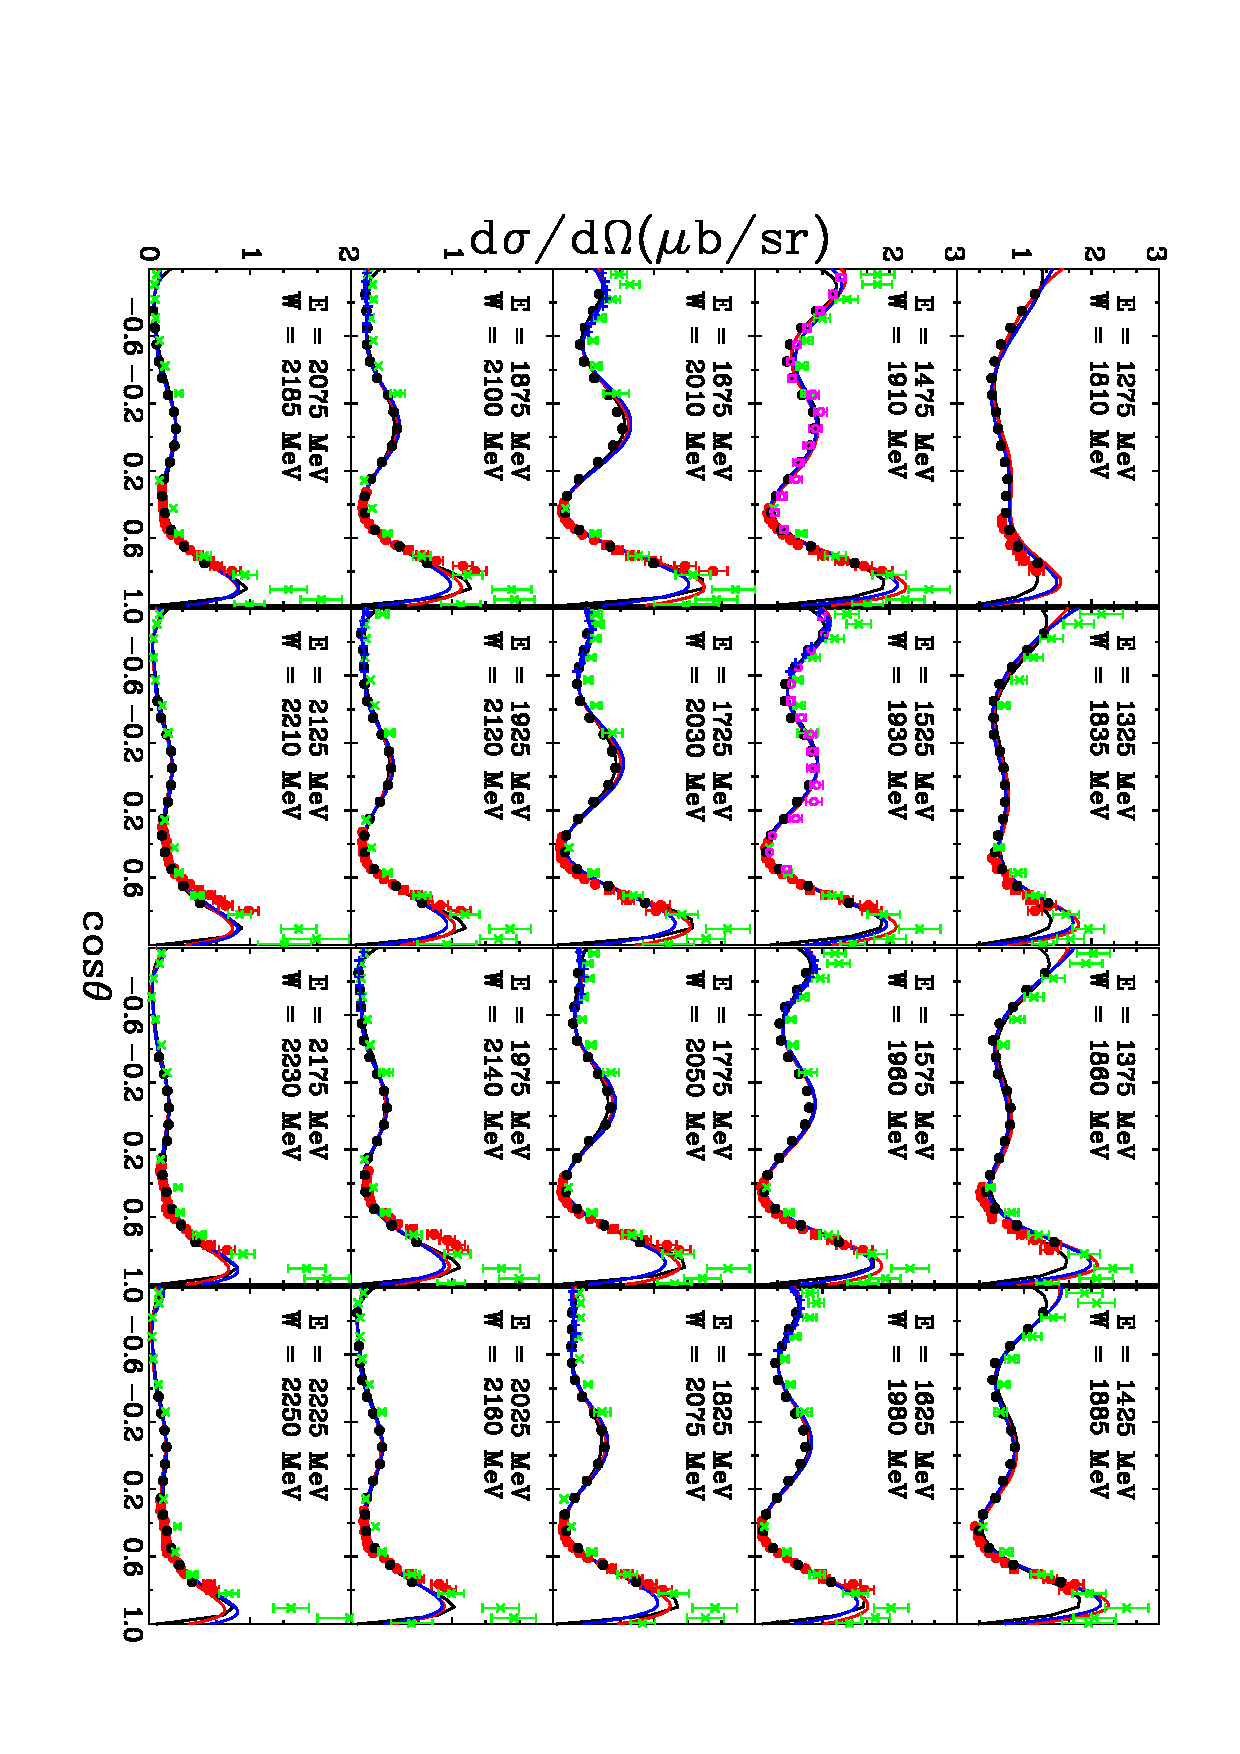
\includegraphics[angle=90,width=\figwidth,height=1.2 \hfigheight]{\figures/analysis/kk01a.pdf}

{Solid lines SAID \textcolor{red}{KU14} \textcolor{blue}{DU13} solution, black solid lines BG2011-02 BnGa predictions. Symbols; \textcolor{red}{this work}, previous \abbr{CLAS}, \textcolor{magenta}{GRAAL}, \textcolor{blue}{LEPS}, \textcolor{green}{CB-ELSA}, previous bremsstrahlung measurements (black open circles).}
\end{center}\end{figure} 
\end{frame}
\begin{frame}
\frametitle{$\cos\theta$ vs. $\frac{d\sigma}{d\Omega}$ (2.275 $\textless$ E$_\gamma$ $\textless$ 3.375 GeV)} 
\begin{figure}[h!]\begin{center}
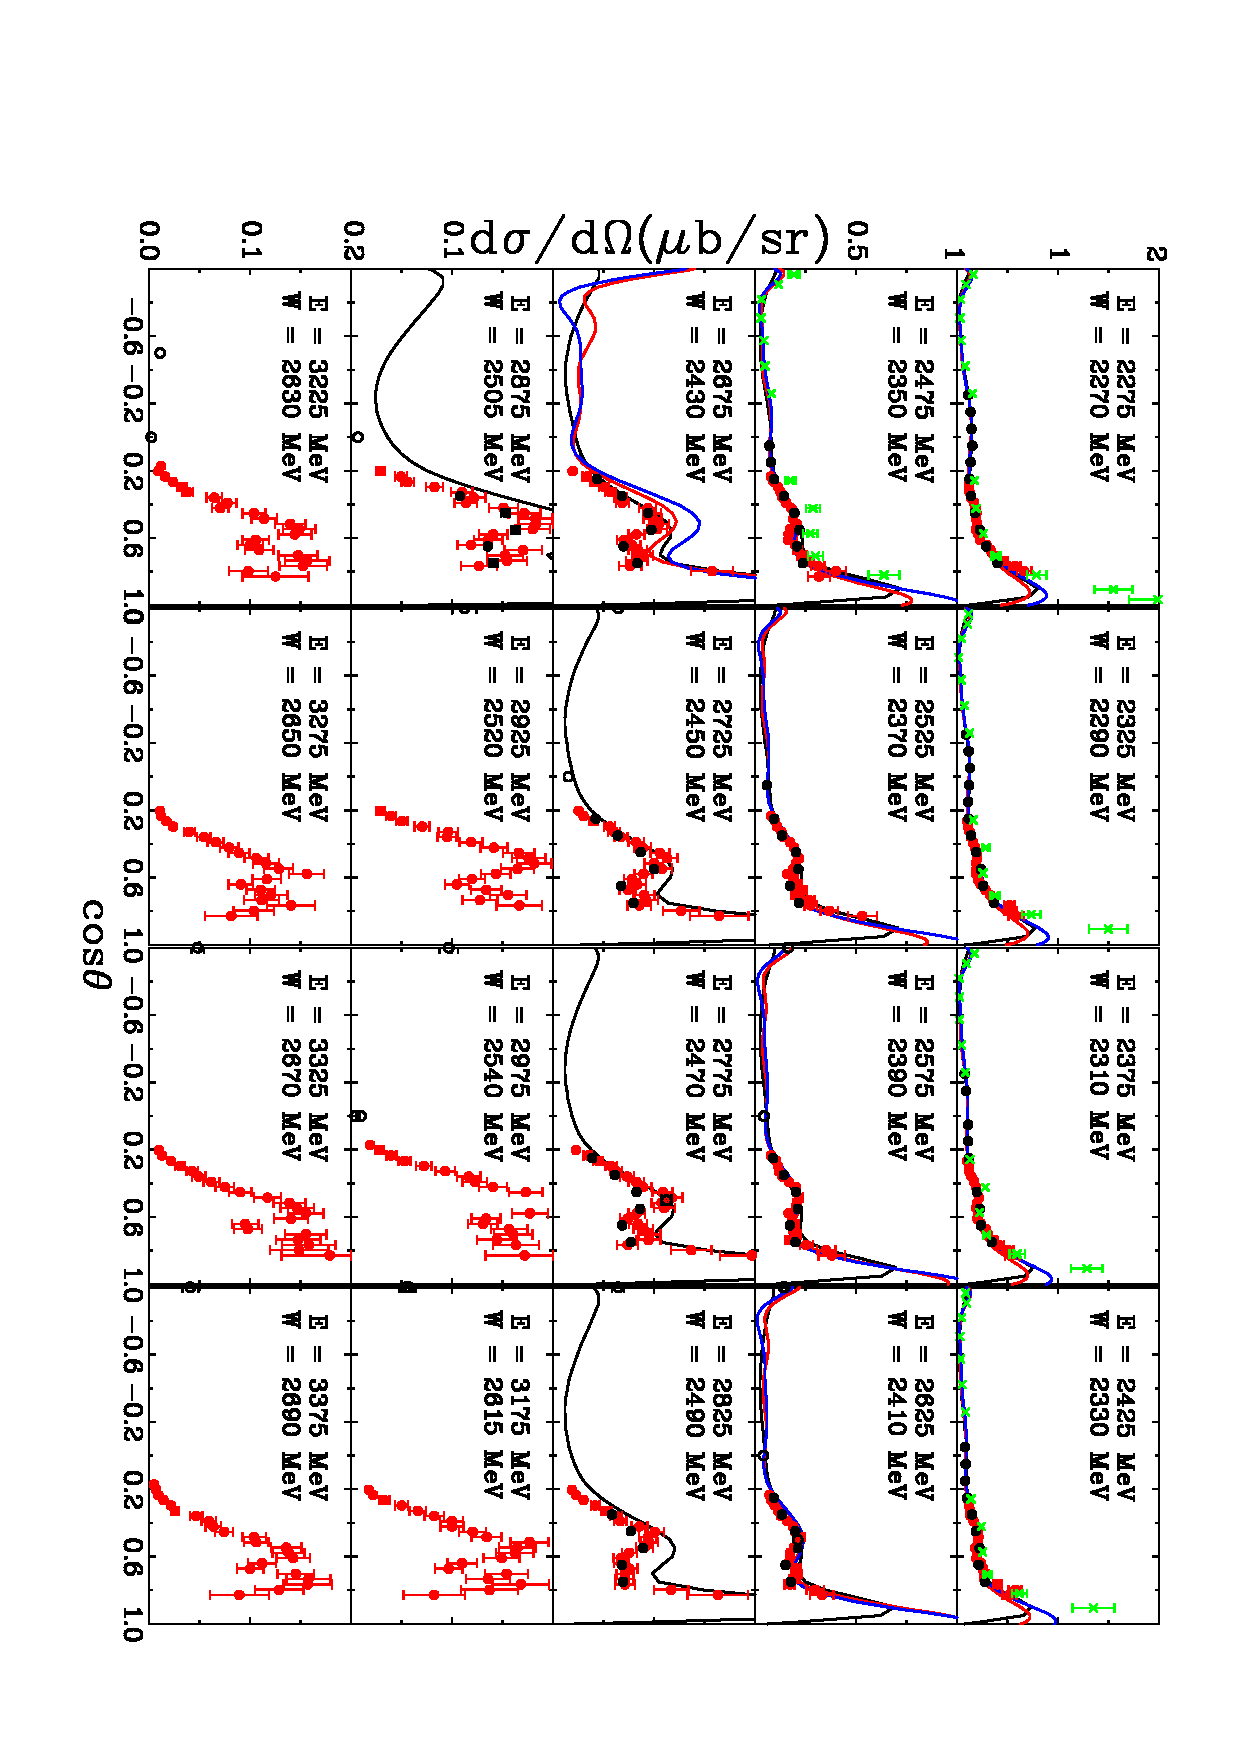
\includegraphics[angle=90,width=\figwidth,height=1.2 \hfigheight]{\figures/analysis/kk02a.pdf}

{Solid lines SAID \textcolor{red}{KU14} \textcolor{blue}{DU13} solution, black solid lines BG2011-02 BnGa predictions. Symbols; \textcolor{red}{this work}, previous \abbr{CLAS}, \textcolor{magenta}{GRAAL}, \textcolor{blue}{LEPS}, \textcolor{green}{CB-ELSA}, previous bremsstrahlung measurements (black open circles).}
\end{center}\end{figure}
\end{frame}
\begin{frame}
\frametitle{$\cos\theta$ vs. $\frac{d\sigma}{d\Omega}$ (3.425 $\textless$ E$_\gamma$ $\textless$ 4.425 GeV)} 
\begin{figure}[h!]\begin{center}
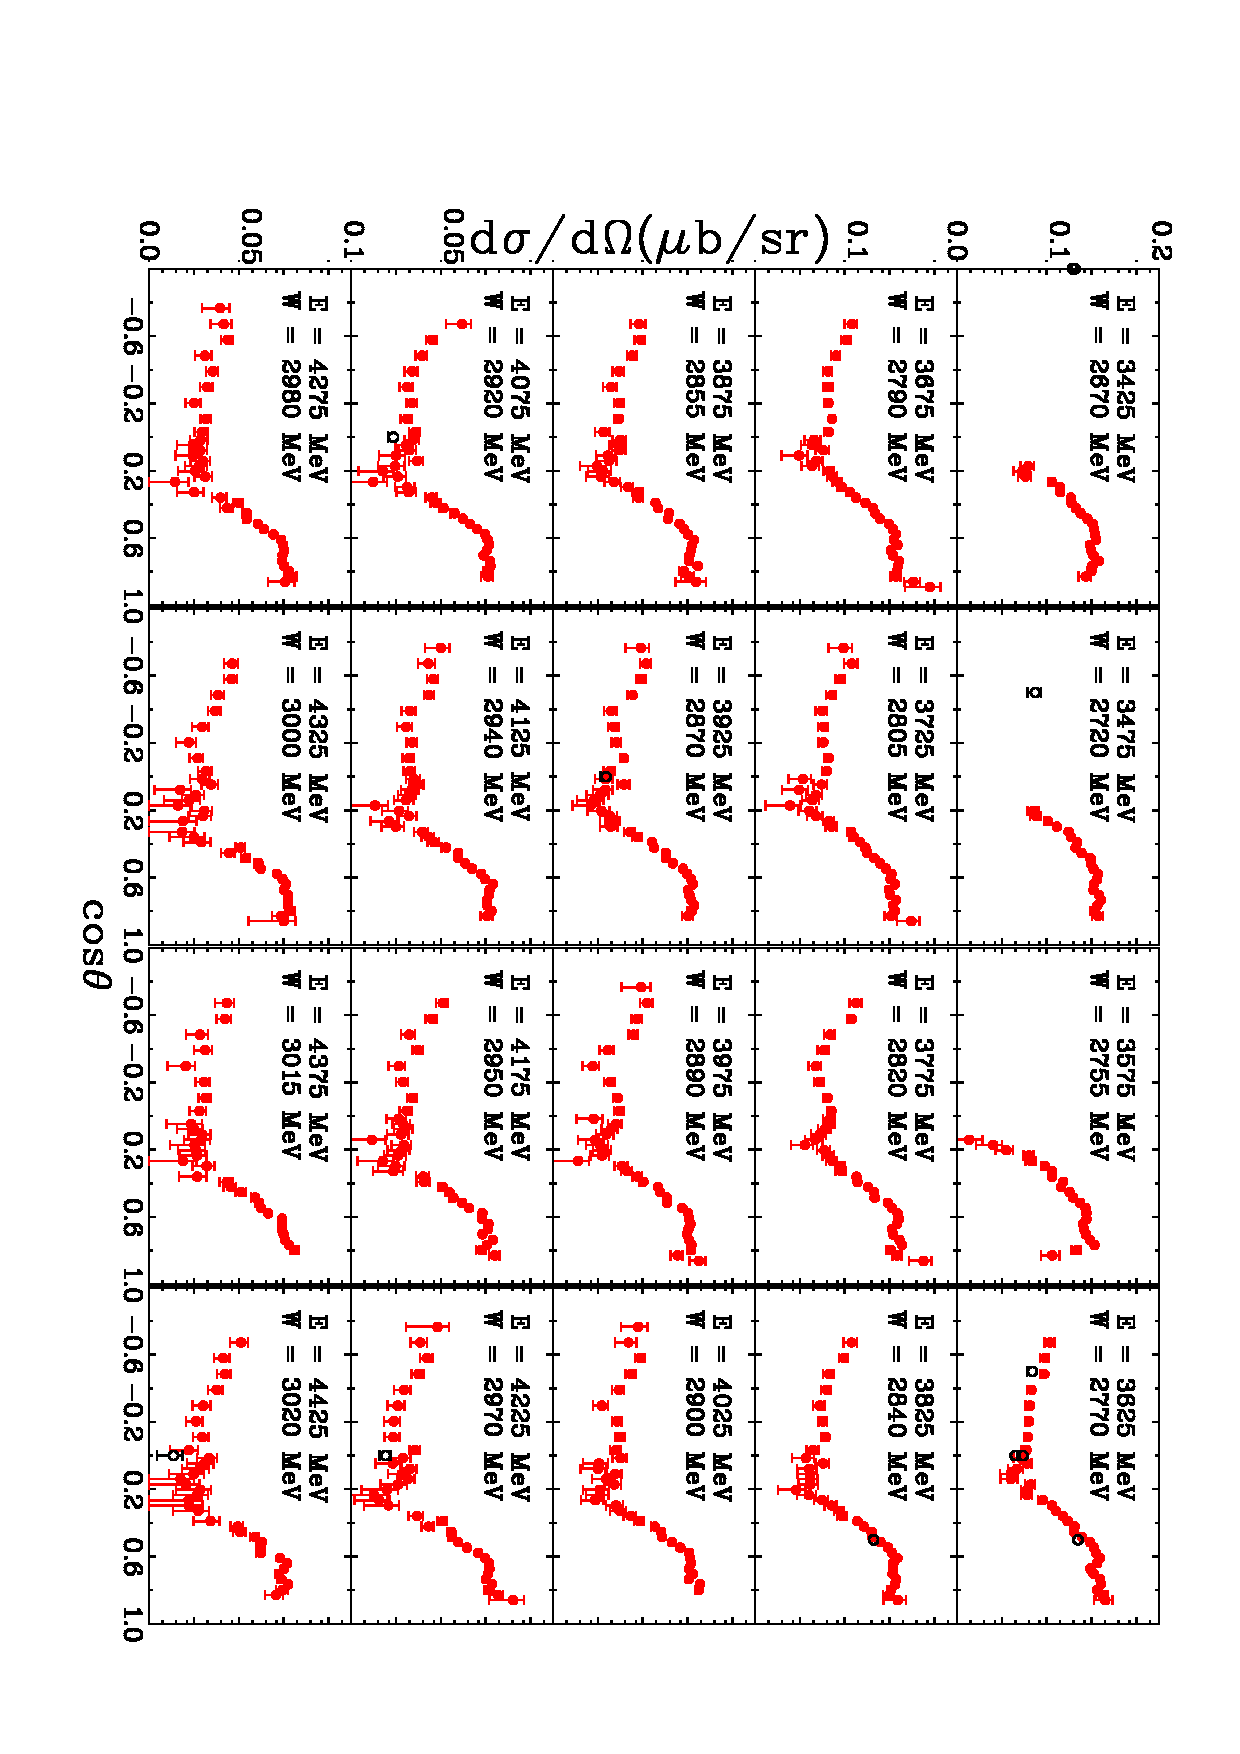
\includegraphics[angle=90,width=\figwidth,height=1.2 \hfigheight]{\figures/analysis/kk03a.pdf}

{Symbols \textcolor{red}{this work}, previous bremsstrahlung measurements (black open circles).}
\end{center}\end{figure}
\end{frame}
\begin{frame}
\frametitle{$\cos\theta$ vs. $\frac{d\sigma}{d\Omega}$ (4.475 $\textless$ E$_\gamma$ $\textless$ 5.425 GeV)} 
\begin{figure}[h!]\begin{center}
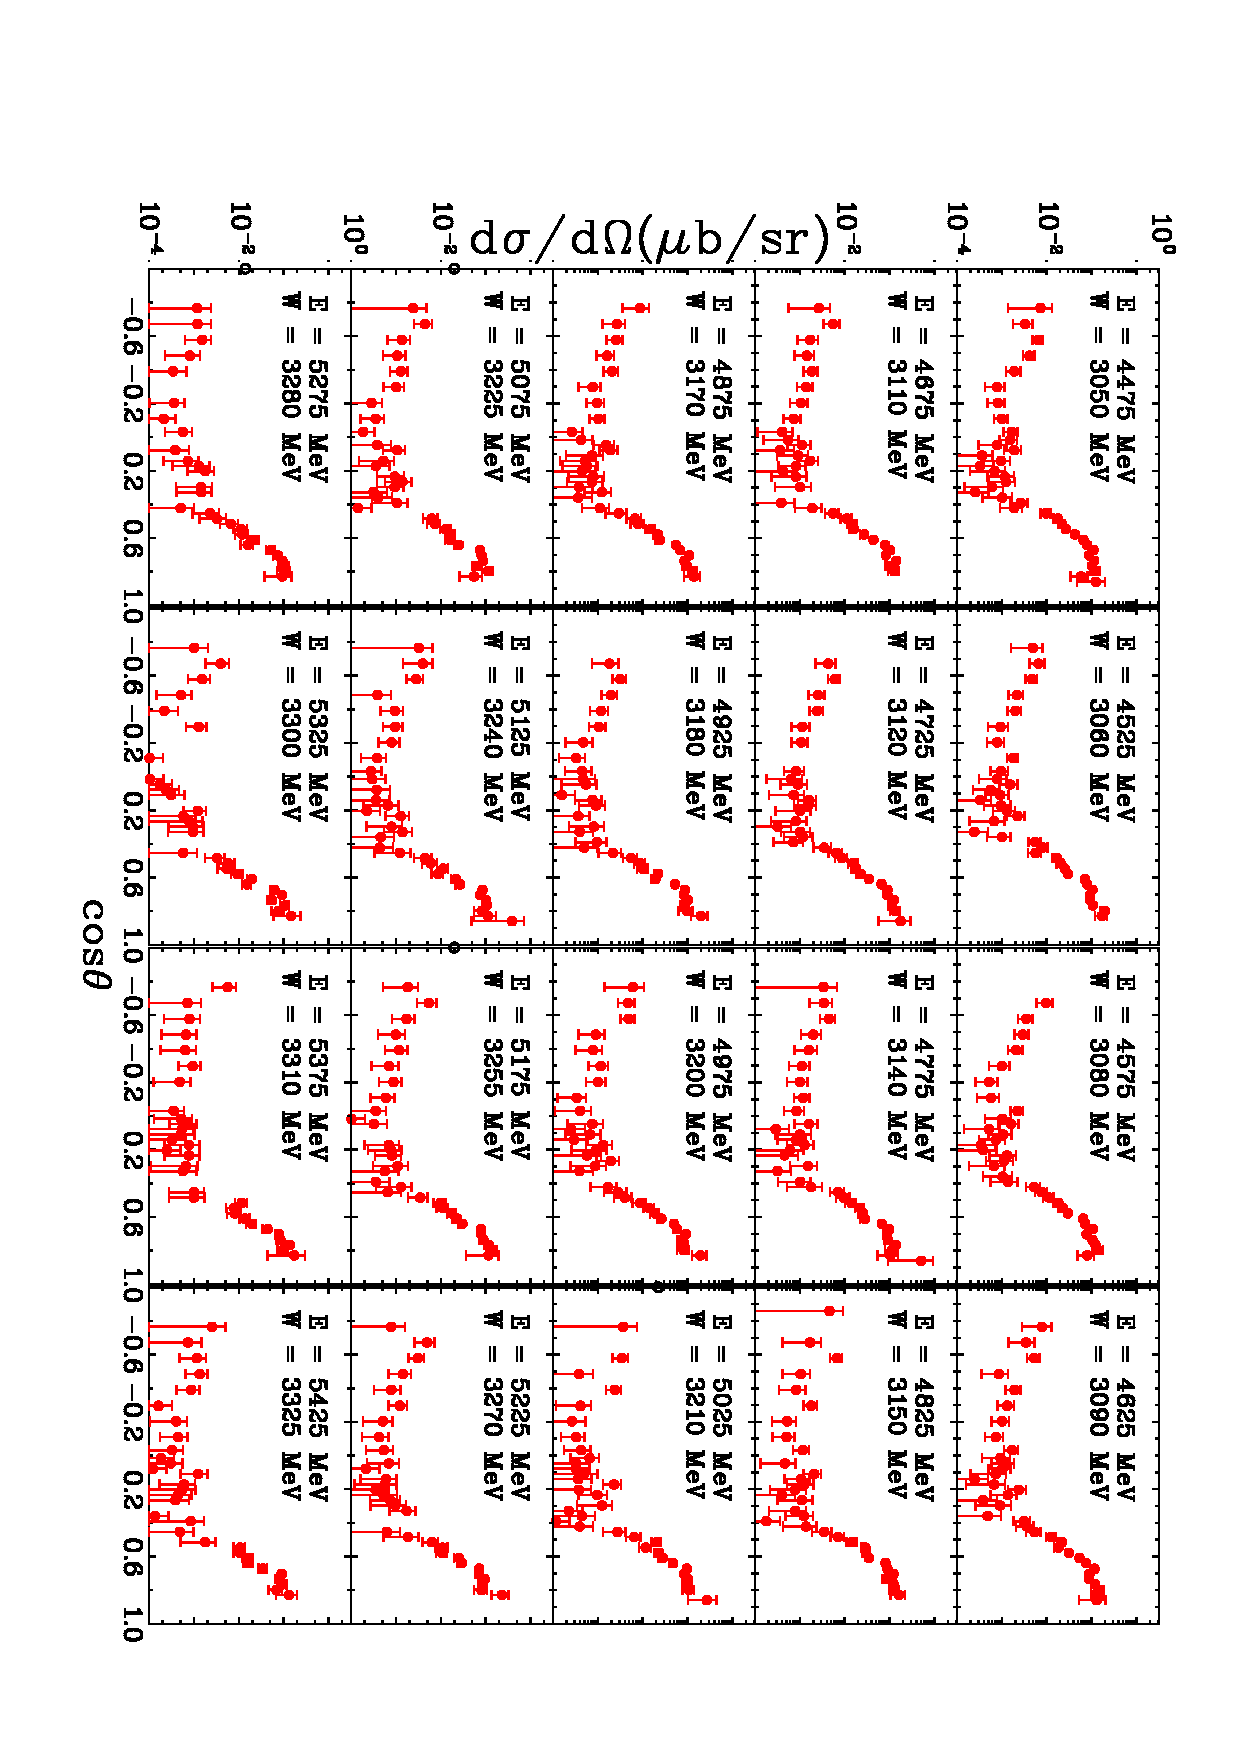
\includegraphics[angle=90,width=\figwidth,height=1.2 \hfigheight]{\figures/analysis/kk04a.pdf}

{Symbols \textcolor{red}{this work}, previous bremsstrahlung measurements (black open circles).}
\end{center}\end{figure}
\end{frame}
%
%
\subsubsection{Differential Cross-Section  $W$ vs. $\frac{d\sigma}{d\Omega}$ }
\begin{frame}
\frametitle{$W$ vs. $d\sigma/d\Omega$ at $\theta$ = 31 -- 75$^\circ$} 
\begin{figure}[h!]\begin{center}
\includegraphics[width=\figwidth,height=1.2 \hfigheight]{\figures/analysis/DSG/mm01a-eps-converted-to.pdf}

{Solid lines SAID \textcolor{red}{KU14} \textcolor{blue}{DU13} solution, black solid lines BG2011-02 BnGa predictions. Symbols; \textcolor{red}{this work}, previous \abbr{CLAS}, previous bremsstrahlung measurements (black open circles).}
\end{center}\end{figure}
\end{frame}
\begin{frame}
\frametitle{$W$ vs. $d\sigma/d\Omega$ at $\theta$ = 76 -- 140$^\circ$} 
\begin{figure}[h!]\begin{center}
\includegraphics[width=\figwidth,height=1.2 \hfigheight]{\figures/analysis/DSG/mm02a-eps-converted-to.pdf}

{Solid lines SAID \textcolor{red}{KU14} \textcolor{blue}{DU13} solution, black solid lines BG2011-02 BnGa predictions. Symbols; \textcolor{red}{this work}, previous \abbr{CLAS}, previous bremsstrahlung measurements (black open circles).}
\end{center}\end{figure}
\end{frame}
\subsubsection{Differential Cross-Section $\left|t\right|$ vs. $\frac{d\sigma}{dt}$}
\begin{frame}
\frametitle{$t$ vs. $d\sigma/dt$ at $E_{\gamma}$ = 1275 -- 2225~MeV } 
\begin{figure}[h!]
\includegraphics[width=\figwidth,height= 1.2 \hfigheight]{\figures/analysis/DSG/kk01b-eps-converted-to.pdf}

{Solid lines SAID \textcolor{red}{KU14} \textcolor{blue}{DU13} solution, black solid lines BG2011-02 BnGa predictions. Symbols; \textcolor{red}{this work}, previous \abbr{CLAS}, \textcolor{magenta}{GRAAL}, \textcolor{blue}{LEPS}, \textcolor{green}{CB-ELSA}, previous bremsstrahlung measurements (black open circles).}
\end{figure}
\end{frame}
\begin{frame}
\frametitle{$t$ vs. $d\sigma/dt$ at $E_{\gamma}$ = 2275 -- 3375~MeV } 
\begin{figure}[h!]
\includegraphics[angle=90,width=\figwidth,height= 1.2 \hfigheight]{\figures/analysis/DSG/kk02b-eps-converted-to.pdf}

{Solid lines SAID \textcolor{red}{KU14} \textcolor{blue}{DU13} solution, black solid lines BG2011-02 BnGa predictions. Symbols; \textcolor{red}{this work}, previous \abbr{CLAS}, \textcolor{magenta}{GRAAL}, \textcolor{blue}{LEPS}, \textcolor{green}{CB-ELSA}, previous bremsstrahlung measurements (black open circles).}
\end{figure}
\end{frame}
\begin{frame}
\frametitle{$t$ vs. $d\sigma/dt$ at $E_{\gamma}$ = 3425 -- 4425~MeV } 
\begin{figure}[h!]
\includegraphics[angle=90,width=\figwidth,height= 1.2 \hfigheight]{\figures/analysis/DSG/kk03b-eps-converted-to.pdf}

{Symbols \textcolor{red}{this work}, previous bremsstrahlung measurements (black open circles).}
\end{figure}
\end{frame}
\begin{frame}
\frametitle{$t$ vs. $d\sigma/dt$ at $E_{\gamma}$ = 4475 -- 5425~MeV } 
\begin{figure}[h!]
\includegraphics[width=\figwidth,height= 1.2 \hfigheight]{\figures/analysis/DSG/kk04b-eps-converted-to.pdf}

{Symbols \textcolor{red}{this work}, previous bremsstrahlung measurements (black open circles).}
\end{figure}
\end{frame}
\begin{frame}
\frametitle{Improvement to Previous SAID Fits}
\begin{figure}[h!]\begin{center}
\includegraphics[width=\figwidth,height= 1.2 \hfigheight]{\figures/analysis/dsg1a-eps-converted-to.pdf}

{\label{fig:chi_sq}Energy dependence of the $\chi^2/dp$ comparison to previous SAID fits, previous \textcolor{blue}{DU13} solution, compared to the new \textcolor{red}{KU14} solution.}
\end{center}\end{figure} 
\end{frame}
\begin{frame}
\frametitle{Comparison with \abbr{GPD} Handbag Model} 
\begin{figure}[h!]\begin{center}
\includegraphics[width=\figwidth,height= 1.2 \hfigheight]{\figures/analysis/DSG/kroll_compare.pdf}

{Differential cross section of $\pi^0$ photoproduction. $E_\gamma = 5.4$~GeV for $s =11$~GeV$^2$. $E_\gamma = 4.8$~GeV for $s =10$~GeV$^2$ \\ Based on this data, a proposal was approved to run in Hall C}
\end{center}\end{figure}
%\begin{itemize}
%\item Based on this data, a proposal was approved to run in Hall C
%\end{itemize}
\end{frame}
\section{Conclusions}
\begin{frame}
\frametitle{Summary and Conclusions} 
\begin{itemize}
\item We measured \piz photoproduction for $\gamma p \to p \pi^0 \to pe^+e^-\gamma$
\item  Data corrections, kinematic fitting and fiducial cuts were used to clean the data $\approx$99\%
\item This data set explained in this analysis is 10\% of the world data for \piz photoproduction
\item More theory is needed to properly explain \piz production at incident photon beam energies higher than 2.8~GeV
\item  Differential cross-sections $\frac{d\sigma}{d\Omega}$ and $\frac{d\sigma}{dt}$, were compared to world data
\item Agreed well $E_\gamma <2.8$~GeV
\item The fits using the SAID parametrization yielded a $\chi^2/dp$ lower than previous existing fits
\item Handbag calculations do not reproduce data for $E_\gamma > 2.8$~GeV
\item Analysis note + paper currently in progress
\end{itemize}
\end{frame}
%\begin{frame}
%\frametitle{Summary and Conclusions} 
%\begin{itemize}
%\item There was a slight discrepancy with the previous limited high energy cross-sections
%\item The fits using the SAID parametrization yielded a $\chi^2/dp$ lower than previous existing fits
%\item The data set explained in this analysis is now 10\% of the world data for \piz photoproduction
%\item More theory is need to properly explain \piz production at incident photon beam energies higher than 2.8~GeV
%\end{itemize}
%\end{frame}
% % % %
% % % %
% % % %
% % % %
% % % %
% % % %
% % % %
% % % %
\begin{frame}
\frametitle{Extras} 
\begin{itemize}
\item Extras are after this $\to$
\end{itemize}
\end{frame}
\begin{frame}
\frametitle{Motivation} 
\begin{itemize}
\item Provide insight into the mechanisms, baryon resonances and productions channels involved in \piz production
\begin{itemize}
\item For incident beam energies already explored previously as well as for incident beam energies in which there exists only a sparse and in some cases no amount of data
\end{itemize}
\item Recently there has been improvement in Wide Angle Compton Scattering predictions using a Generalized Parton Distribution (\abbr{GPD}) handbag model.
\begin{itemize}
\item This framework has also been recently adopted into \piz production
\item The production of the nucleons is considered in a 2 part soft and hard mechanism exchange
\end{itemize} 
\item Goal is to provide precise measurements of the \piz cross-section 
\begin{itemize}
\item Compare to existing data
\item Check validity of handbag model
\end{itemize}
\end{itemize}
\end{frame}
\begin{frame}
\frametitle{\piz Production below 2.8~GeV}  
\begin{figure}[h!]\begin{center}
\includegraphics[width=0.75 \figwidth,height=0.9\qfigheight]{\figures/mike_defense_III.pdf}
\end{center}\end{figure}
\begin{align}
\mathcal{M} = [\frac{1}{2}i\gamma_5\gamma_{\mu}\gamma_{\nu}A_{1}(s,t) + 2i\gamma_5P_\mu(q-\frac{1}{2}k)_\nu A_2(s,t) & \nonumber \\ \nonumber  + \gamma_5\gamma_{\mu}q_{\nu}A_{3}(s,t) + \gamma_5\gamma_{\mu}(2P_\nu-iM\gamma_\nu)A_{4}(s,t)]& (\epsilon_\mu k_\nu - \epsilon_\nu k_\mu) \nonumber
\end{align}
\begin{itemize}
\item $q_\mu$ and $k_\nu$ are the four-momenta of the $\pi^0$ and photon respectively
\item $P_\mu = \frac{1}{2}(p_{1\mu}+p_{2\nu})$
\item $\epsilon_\mu \equiv$ photon polarization 
\end{itemize}
\end{frame}
\begin{frame}
\frametitle{\piz Production below 2.8~GeV} 
\begin{itemize}
\item The \piz cross-section can be reconstructed by electric $(E_{l\pm})$ and magnetic $(M_{l\pm})$ multipole amplitudes 
\begin{itemize}
\item  $l$ is angular momentum of the final state with total angular momentum $ j=l\pm \frac{1}{2}$
\end{itemize}
\item Isospin Decomposition
\begin{itemize}
\item The photon interaction has an isovector part and isoscalar part
\item The isovector photon produces final states with isospin $\frac{3}{2}$ and $\frac{1}{2}$ with amplitudes $A^{V3}$ and $A^{V1}$
\item The isoscalar photon gives final states of isospin $\frac{1}{2}$ with amplitude $A^S$.
\item $\pi^0: A^0 = \sqrt{\frac{2}{3}} A^{V3} + \sqrt{\frac{1}{3}}(A^{V1}-A^{S})$
\end{itemize}
\item Helicity Partial-Wave Amplitudes
\item \abbr{CGLN} Amplitudes
\end{itemize}
\end{frame}
\begin{frame}
\frametitle{\piz Production above 2.8~GeV} 
\begin{itemize}
\item \piz production is factorized into two parts
\begin{itemize}
\item one quark from the incoming and one from the outgoing nucleon participate in the hard sub-process (small blob)
\begin{itemize}
\item calculable using \abbr{pQCD}
\end{itemize}
\item The soft part consists of all the other partons that are spectators and can be described in terms of GPDs (large blob)
\end{itemize}
\end{itemize}
\begin{figure}[h!]\begin{center}
\includegraphics[width= \figwidth ,height=0.75 \hfigheight]{\figures/intro/handbag.pdf}
\caption[Handbag Diagram for Photoproduction]{\label{fig:xsection.handbag}	The handbag-type diagram for photoproduction of mesons.}
\end{center}\end{figure}
\end{frame}
\begin{frame}
\frametitle{\piz Production above 2.8~GeV} 
\begin{itemize}
\item Recent framework of handbag model led to \piz cross-section predictions
\end{itemize}
\begin{figure}[h!]\begin{center}
\includegraphics[width=\figwidth ,height=\hfigheight]{\figures/intro/photo-fig7.pdf}
\caption[Theoretical Cross-Section for \piz at High Energies ]{\label{fig:xsection.handbag.cal}The soft physics contribution to the cross-section for photoproduction of \piz scaled by s$^7$ versus $\cos\theta$, where $\theta$ is the scattering angle in the $\gamma p$ c.m. system.}
\end{center}\end{figure}

\end{frame}
\begin{frame}
\frametitle{SAID} 
\begin{itemize}
\item SAID is a repository of experimental data and an interactive analysis facility
\begin{itemize}
\item Allows to compare and extract data and partial wave solutions (\abbr{PWA}) for a variety of photoproduction, electro-production and pion production reactions
\end{itemize}
\item SAID generates resonance couplings, in terms of angular momentum and isospin quantum numbers
\begin{itemize}
\item Extracted from a fit-based determination of multipoles using both an energy-dependent and an energy-independent parametrization
\end{itemize}
\end{itemize}
\end{frame}
\begin{frame}
\frametitle{\piz$\to \gamma^{(\star)}(\epsilon_1,p) \gamma(\epsilon_2,k)$ Decay} 
\begin{itemize}
\item The \piz decays to 2 photons $98.823 \pm 0.034 \%$
\begin{itemize}
\item Each photon has equal probability of pair producing \epem pairs
\end{itemize}
\item The \piz decays to \epem $\gamma$ $1.174 \pm0.035 \%$
\end{itemize}
\begin{figure}[h!]\begin{center}
\includegraphics[width=\figwidth,height=0.75\hfigheight]{\figures/intro/decays/Hydrogen_conversion_Prob_4Photons.pdf}
\caption[Pair Production Through Liquid Hydrogen]{\label{fig:conversion}{Probability of \emph{pair production}, $\gamma \to$\epem, in 40~cm of liquid hydrogen.}}
\end{center}\end{figure}
\end{frame}
\begin{frame}
\frametitle{CLAS Detector}
\begin{figure}[h!]\begin{center}
\includegraphics[width=\figwidth,height=1.5 \hfigheight]{\figures/hall-b/clas_schematic.pdf}
\caption[Pair Production Through Liquid Hydrogen]{\label{fig:clas}{CLAS Detector with labeling}}
\end{center}\end{figure}
\end{frame}
\begin{frame}
\frametitle{Photon Beam}
\begin{itemize}
\item Bremsstrahlung photon beam\\
\begin{itemize}\addtolength{\itemsep}{0.5\baselineskip}
\item e$^-$ beam of 5.7 GeV\\
\item gold radiator 10$^{-4}$ radiation lengths\\
\item Tagged $\gamma$ energies 1.1 $\rightarrow$ 5.5 GeV\\
\item 6.2 mm diameter collimator 537 cm before $\ell H_{2}$ target\\
\end{itemize}
\end{itemize}
\end{frame}
\begin{frame}
\frametitle{Liquid Hydrogen $\ell H_2$ Target}
\begin{itemize}
\item Liquid Hydrogen $\ell H_2$ Target\\
\begin{itemize}\addtolength{\itemsep}{0.5\baselineskip}
\item Unpolarized\\
\item 40 cm in length\\
\item 2 cm radius
\begin{itemize}
\item $\gamma$ beam had 1.5 cm radius exiting $\ell H_{2}$ target\\
\end{itemize}
\item Placed 90 cm upstream from CLAS center \\
\begin{itemize}\addtolength{\itemsep}{0.5\baselineskip}
\item Geometric acceptance of 6$^{\circ}$ instead of 8$^{\circ}$ in lab frame \\
\item Geometric acceptance of 100$^{\circ}$ instead of 140$^{\circ}$ in lab frame \\
\end{itemize}
\end{itemize}
\end{itemize}
\end{frame}
\begin{frame}
\frametitle{$e^{+}e^{-}$ Identification}
\begin{itemize}\addtolength{\itemsep}{0.5\baselineskip}
\item CC's were filled with perflourbutane $C_{4}F_{10}$
\begin{itemize}\addtolength{\itemsep}{0.5\baselineskip}
\item Index of refraction 1.0015
\item $\pi^{\pm}$ threshold of 2.7 GeV
\item $e^{\pm}$ threshold of 9 MeV
\item $e^{\pm}$ detection efficiency > 97\% for charged particles below 2.5 GeV.
\end{itemize}
\end{itemize}
\end{frame}
\begin{frame}
\frametitle{Discerning between $e^{\pm}$ and $\pi^{\pm}$}
\begin{small}
\begin{columns}
\begin{column}{4.5cm}
\begin{itemize}\addtolength{\itemsep}{0.5\baselineskip}
\item $e^{\pm}$ trigger
\begin{itemize}\addtolength{\itemsep}{0.5\baselineskip}
\item Single track (ST*TOF)*(EC*CC)
\item L2 multiplicity of 2.
\begin{itemize}\addtolength{\itemsep}{0.5\baselineskip}
\item 2 tracks were detected in the Drift Chambers
\end{itemize}
\item  Trigger bit was set to be 6 of 12
\end{itemize}
\end{itemize}
\end{column}
\begin{column}{4.5cm}
\begin{figure}[h]
\begin{center}
\includegraphics[height=4.6cm,width=4.5cm]{\figures/analysis/run57130_Twolep_normalizedII.pdf}
\caption{Triggers fired for leptons}
\end{center}
\end{figure}
\end{column}
\end{columns}
\end{small}
\end{frame}
\begin{frame}
\frametitle{Overview }
\begin{small}
\begin{columns}
\begin{column}{4.5cm}
\begin{itemize}
\item Data was taken in Hall B experiment G12
\item Running Time: 04/2008 $\rightarrow$ 06/2008
\item 44 Days of Beam Time
\item 60 - 65 nA of current
\item E$_{\gamma}$ up to 5.5 GeV
\item 126 TB Raw Data
\end{itemize}
\end{column}
\begin{column}{4.5cm}
\begin{itemize}
\item Raw sensitivity of ~ 53 pb$^{-1}$
\item 26.2 x10$^{9}$ production triggers (3 x 10$^{6}$ di-lepton triggers)
\item EC and CC combine to provide an e/$\pi$ rejection factor of 10$^{-6}$ for di-lepton pairs.
\item $\frac{\Gamma_{e^+e^-\gamma}}{\Gamma_{\pi^+\pi^-\gamma}} = 	0.237 � 0.026   $
\end{itemize}
\end{column}
\end{columns}
\end{small}
\end{frame}
\begin{frame}
\frametitle{Energy Loss (ELoss)} 
\begin{itemize}
\item Tracking begins after the particle had already traversed through the target and \abbr{ST}
\begin{itemize}
\item Momentum determination was skewed by the ``energy-loss'' the particle underwent before entering Region 1
\item ``Energy-loss' is due to charged particles losing their energy through atomic excitation and ionization while traveling through materials in the \abbr{CLAS} detector
\item Leptons such as electrons/positrons or muons are not subjective to ``energy-loss''.
\end{itemize}
\item Eloss software package written by Eugene Pasyuk for the CLAS detector has been implemeted in this analysis
\end{itemize}
\end{frame}
\begin{frame}
\frametitle{Beam Corrections} 
\begin{itemize}
\item First noticed by \g12 participants at the analysis level in which M$_x$($\pi^+\pi^-$) and M$_x$($\pi^+\pi^-\pi^+$) masses were systematically low. Varied in mass as much as 10~MeV.
\item Dependent on the run number
%\item Varied in mass as much as 10~MeV.
\end{itemize}\vspace{-1.2em}
\begin{figure}
     \centering
     \subfigure{\includegraphics[width=\figwidth,height=0.75\hfigheight]{\figures/analysis/beam_correction/P_mass_issue.pdf}}\vspace{-1.5em}
     \subfigure{\includegraphics[width=\figwidth,height=0.75\hfigheight]{\figures/analysis/beam_correction/N_mass_issue.pdf}}
     \caption{Plot of \g12 run number vs. proton(neutron) top(bottom) mass with and without the ``energy-loss'' applied. \abbr{PDG} mass for the proton(neutron) is 0.938272 (0.939565) GeV/c.}
\end{figure}

\end{frame}
\begin{frame}
\frametitle{Beam Corrections} 
\begin{itemize}
\item Investigated invariant mass of M($\pi^+\pi^-$) = M$_{K_s}$ for run number dependence
\begin{itemize}
\item Dependent on the run number was not found
\end{itemize}
\end{itemize}
\begin{figure}[h!]\begin{center}
\includegraphics[width=\figwidth,height=0.75\hfigheight]{\figures/analysis/beam_correction/Kaon_mass.pdf}
\caption[Kaon Mass for Run 56515 and 57130]{\label{fig:beamcor.k_mass}Plot of Kaon mass for runs 56515 and 57130.  \abbr{PDG} mass for the kaon is 0.497614 GeV/c.}
\end{center}\end{figure}
\end{frame}
\begin{frame}
\frametitle{Beam Corrections} 
\begin{itemize}
\item Problem was associated with the beam
\item Tagger y-dump positioning changed 
\begin{itemize}
\item \g12 performed shut down midway. Upon restart the tagger magnet was also restarted
\end{itemize}
\end{itemize}
\begin{figure}[h!]\begin{center}
\includegraphics[width=\figwidth,height=0.75\hfigheight]{\figures/analysis/beam_correction/600px-Tagger-dump-y.pdf}
\caption[Tagger Dump Y-Positioning]{\label{fig:tagdump}Tagger dump y-positioning according to \abbr{EPICS}}
\end{center}\end{figure}
\end{frame}
\begin{frame}
\frametitle{Beam Corrections} 
\begin{itemize}
\item Problem identified as hysteresis in the tagger magnet
\end{itemize}
\begin{figure}[h!]\begin{center}\vspace{-1em}
\includegraphics[width=\figwidth,height=1.3 \hfigheight]{\figures/analysis/beam_correction/hysteresis_keynote.pdf}
\caption[Plot Depicting the Process of Hysteresis]{\label{fig:hyst}Plot depicting the process of hysteresis. For the a current of strength I, there could exist two magnetic fields of strength B.}
\end{center}\end{figure}
\end{frame}
\begin{frame}
\frametitle{Beam Correction} 
\begin{itemize}
\item $(P_{\gamma} + P_{target} - (P_{\pi^+\pi^-}))^2 = m_p^2$
\item $P_{\pi^+\pi^-}^2 - 2P_{target}P_{\pi^+\pi^-}= 2P_{\gamma}(P_{\pi^+\pi^-} - P_{target})$
\item $P_{\gamma} = P_{E_0} - P_{e}$
\begin{itemize}
\item $P_{E_0}$ beam energy delivered from \abbr{CEBAF}
\item $P_e$ scattered electron in the \emph{bremsstrahlung} process that is recorded by the tagger
\end{itemize}
\item Correction factor
\begin{itemize}
\item $x= \frac{P_{E_0}(P_{target}-P_{\pi^+\pi^-}) + P_{\pi^+\pi^-}^2/2  - P_{target}P_{\pi^+\pi^-}}{(P_{E_0} - P_{\gamma})(P_{target} - P_{\pi^+\pi^-})}$
\end{itemize}\vspace{1em}
\item $P_{\gamma}^{new} = P_{E_0} - P_e*x$
\end{itemize}
\end{frame}
\begin{frame}
\frametitle{Beam Correction} 
\begin{itemize}
\item Value of x was obtained for each run
\item Applied correction to the topology $\gamma p \to \pi^+\pi^+\pi^-(n)$
\end{itemize}
\begin{figure}[h!]\begin{center}
\includegraphics[width=\figwidth,height=0.9\hfigheight]{\figures/analysis/beam_correction/C3pi_allcorr_neutron_rxr.pdf}
\caption[Corrected Missing Neutron Mass for \g12 Using Beam Corrections]{\label{fig:neutron.fixall} Plot of missing neutron mass using various corrections.}
\end{center}\end{figure}
\end{frame}
\begin{frame}
\frametitle{Geometric Fiducial Cuts} 

\begin{figure}
     \centering
     \subfigure{\includegraphics[width=\figwidth,height=0.75\hfigheight]{\figures/analysis/FIDUCIAL_CUTS/GEOMETRIC/pip_theta_cos_sin_phi_nofid.pdf}}\vspace{-1.5em}
     \subfigure{\includegraphics[width=\figwidth,height=0.75\hfigheight]{\figures/analysis/FIDUCIAL_CUTS/GEOMETRIC/pip_theta_cos_sin_phi_wfid.pdf}}
     \caption{Positive charged tracks in \abbr{CLAS} \abbr{DC} before and after fiducial cut being applied}
\end{figure}

\end{frame}
\begin{frame}
\frametitle{Geometric Fiducial Cuts} 
\begin{figure}
     \centering
     \subfigure{\includegraphics[width=\figwidth,height=0.75\hfigheight]{\figures/analysis/FIDUCIAL_CUTS/GEOMETRIC/pim_theta_cos_sin_phi_nofid.pdf}}\vspace{-1.5em}
     \subfigure{\includegraphics[width=\figwidth,height=0.75\hfigheight]{\figures/analysis/FIDUCIAL_CUTS/GEOMETRIC/pim_theta_cos_sin_phi_wfid.pdf}}
     \caption{Negative charged tracks in \abbr{CLAS} \abbr{DC} before and after fiducial cut being applied}
\end{figure}

\end{frame}
\begin{frame}
\frametitle{EC Fiducial Cuts} 
\begin{itemize}
\item EC dead/inefficient \abbr{PMT}'s were found and removed
\end{itemize}
\begin{figure}[h!]\begin{center}
\includegraphics[width=\figwidth,height=\hfigheight]{\grpath/analysis/FIDUCIAL_CUTS/EC/pim_ecuvw_phi_NOKnockout_sec5.pdf}
\caption[Inefficient \abbr{EC} U, V, W strips vs. $\phi$ for Sector 5]{\label{fig:neg:ec.sec5}Inefficiency seen in \abbr{CLAS} $e^{-} \ $ data, due to an inefficient \abbr{EC} strips. Top row depicts the U, V, W strips for the \emph{inner} \abbr{EC}, while the bottom row depicts the U, V, W strips for the \emph{outer} \abbr{EC}}
\end{center}\end{figure}
\end{frame}
\begin{frame}
\frametitle{EC Fiducial Cuts} 
\begin{itemize}
\item EC sectors 1, 2, 3, 5 had dead/inefficient \abbr{PMT}'s. Sector 5 was the worst 
\end{itemize}
\begin{figure}[h!]\begin{center}
\includegraphics[width=\figwidth,height=\hfigheight]{\grpath/analysis/FIDUCIAL_CUTS/EC/pim_ecuvw_phi_afterGeoFid_sec5.pdf}
\caption[\abbr{EC} U, V, W strips vs. $\phi$ for Sector 5 with Fiducial Cuts]{\label{fig:neg:ec.sec5_cut} Plot depicting fiducial cuts and ineffcient paddle knockouts applied to $e^-$ data. Top row depicts the U, V, W strips for the \emph{inner} \abbr{EC}, while the bottom row depicts the U, V, W strips for the \emph{outer} \abbr{EC}}
\end{center}\end{figure}
\end{frame}
\begin{frame}
\frametitle{\abbr{TOF} Fiducial Cuts} 
\begin{itemize}
\item Sector 1 and 3 had dead/ineffcient \abbr{TOF} paddles
\item Performing a geometric cut on is same as cutting dead paddles
\end{itemize}
\begin{figure}[h!]\begin{center}
\includegraphics[width=\figwidth,height=\hfigheight]{\grpath/analysis/FIDUCIAL_CUTS/TOF/RAW/pip_sec3.pdf}
\caption[Positive Charge Particle \abbr{TOF} Inefficiency Plot for Sector 3]{\label{fig:pos:tofcut_off}Inefficiency seen in \abbr{CLAS} $\pi^{+} \ $ data, due to an inefficient \abbr{TOF} paddle.}
\end{center}\end{figure}
\end{frame}
\begin{frame}
\frametitle{\abbr{TOF} Fiducial Cuts} 
\begin{figure}[h!]\begin{center}
\includegraphics[width=\figwidth,height=\hfigheight]{\grpath/analysis/FIDUCIAL_CUTS/TOF/KNOCK_OUT/pip_sec3_Knockout.pdf}
\caption[Positive Charge Particle \abbr{TOF} Inefficiency Cut Plot for Sector 3]{\label{fig:pos:tofcut_on}Inefficiency cut for $\pi^{+} \ $ and proton data.}
\end{center}\end{figure}
\end{frame}
\begin{frame}
\frametitle{Simulation}
\begin{itemize}
\item Simulation Chain
\begin{itemize}
\item PLUTO++ as generator
\item \abbr{GAMP2PART}
\item \abbr{GSIM}
\item \abbr{GPP}
\item \abbr{A1C}
\item \abbr{Analysis Code}
\end{itemize} 
\end{itemize}
\end{frame}
\begin{frame}
\frametitle{Lepton Trigger Simulation} 
\begin{itemize}
\item Lepton triggered was simulated by
\begin{itemize}\label{trig:sim.all}
\item The sector with the highest EC summed energy over threshold. \label{trig:sim.ECtot} 
\item The sector with the highest EC Inner Layer summed energy over threshold. \label{trig:sim.ECinner} 
\item The sector with the highest CC summed energy over threshold. \label{trig:sim.CCtot} 
\item All three above conditions must be in same sector.
\end{itemize}
\item This procedure is how data is triggered in \g12
\item Simulating the trigger in conjunction with \abbr{CC} and \abbr{EC} hit requirements reduced the yield of the simulation to 69.48\% while for the data the reduction is 69.91\% 
\end{itemize}
\end{frame}
\begin{frame}
\frametitle{Simulation Verification} 
\begin{itemize}
\item Real data was inputted into \abbr{GSIM}
\item Initially had success rate of 0.75\% due to \abbr{GSIM} \abbr{CC} and \abbr{EC} pedestal values at reconstruction
\item A special \abbr{CLAS\_CALDB\_RUNINDEX} was created for leptons and photons after which $\approx$~95~\% success
\item Missing 5\% is start-couter failure seen in both \abbr{MC} and data due to sector random bug
\end{itemize}
\begin{figure}[h!]\begin{center}
\includegraphics[width=\figwidth,height=0.75\hfigheight]{\grpath/hall-b/st_issue_4_thesis.pdf}
\caption[Start Counter Inefficiency]{\label{fig:classt.ineffII}{\coloronline}Start counter inefficiency}
\end{center}\end{figure}
\end{frame}
\begin{frame}
\frametitle{Kinematic Fitting}
\begin{itemize}
\item $\eta = y + \epsilon$
\begin{itemize}
\item Use of Lagrange multipliers and least-squares fitting 
\end{itemize}\vspace{0.25cm}
\item $P(\chi^2)=\int^{\infty}_{\chi^2}f(x,n)dx $
\begin{itemize}
\item $f(x,n) \equiv \chi^2$ probability density function for $n$ degrees of freedom
\item $0<P(\chi^2)<1$ 
\end{itemize}\vspace{0.25cm}
\item $\vec{z} = \frac{\vec{\eta_i} - \vec{\eta_f}}{\sqrt{\sigma_{\vec{\eta_i}}^2 - \sigma_{\vec{\eta_f}}^2}} $
\end{itemize}
\end{frame}
\begin{frame}
\frametitle{Kinematic Fitting} 
\begin{figure}[h!]\begin{center}
\includegraphics[width=\figwidth,height= 1.2 \hfigheight]{\figures/analysis/KineFitter/Lep_Pulls_fix.pdf}
\caption[Lepton Pull Parameters for Kinematic Fitting Using Data]{\label{fig:kinfit.LepPullData}Pull distribution for the (4-C) kinematic fit for $\gamma p \rightarrow p e^+ e^-$ for \g12 data with a 1\% Confidence Level cut applied, and a Gaussian fit to each.}
\end{center}\end{figure}
\end{frame}
\begin{frame}
\frametitle{Kinematic Fitting} 
\begin{figure}[h!]\begin{center}
\includegraphics[width=\figwidth,height=  1.2  \hfigheight]{\figures/analysis/KineFitter/Lep_Pulls_MC.pdf}
\caption[Lepton Pull Parameters for Kinematic Fitting Using Monte-Carlo]{\label{fig:kinfit.LepPullMC}Pull distribution for the (4-C) kinematic fit for $\gamma p \rightarrow p e^+ e^-$ for \g12 simulation with a 1\% Confidence Level cut applied, and a Gaussian fit to each.}
\end{center}\end{figure}
\end{frame}
\begin{frame}
\frametitle{Kinematic Fitting} 
\begin{figure}[h!]\begin{center}
\includegraphics[width=\figwidth,height=  1.2  \hfigheight]{\figures/analysis/KineFitter/GP_PEpEm_PullProbThesis.pdf}
\caption[Lepton Pull Probabilities for Kinematic Fitting]{\label{fig:kinfit.LepPullProb}Confidence Level for \g12 (top) data and \g12 simulation (bottom) for a (4-C) fit using $\gamma p \rightarrow p e^+ e^-$}
\end{center}\end{figure}
\end{frame}
\begin{frame}
\frametitle{Kinematic Fitting} 
\begin{figure}[h!]\begin{center}
\includegraphics[width=\figwidth,height=  1.2  \hfigheight]{\figures/analysis/KineFitter/GP_PPipPim_PullsThesis.pdf}
\caption[Pion Pull Parameters for Kinematic Fitting Using Data]{\label{fig:kinfit.PiPullData}Pull distribution for the (4-C) kinematic fit for $\gamma p \rightarrow p \pi^+ \pi^-$ for \g12 data with a 1\% Confidence Level cut applied, and a Gaussian fit to each.}
\end{center}\end{figure}
\end{frame}
\begin{frame}
\frametitle{Kinematic Fitting} 

\begin{figure}[h!]\begin{center}
\includegraphics[width=\figwidth,height=  1.2  \hfigheight]{\figures/analysis/KineFitter/GP_PPipPim_PullsThesis_MC.pdf}
\caption[Pion Pull Parameters for Kinematic Fitting Using Monte-Carlo]{\label{fig:kinfit.PiPullMC}Pull distribution for the (4-C) kinematic fit for $\gamma p \rightarrow p \pi^+ \pi^-$ for \g12 simulation with a 1\% Confidence Level cut applied, and a Gaussian fit to each.}
\end{center}\end{figure}
\end{frame}
%
\begin{frame}
\frametitle{Kinematic Fitting} 
\begin{figure}[h!]\begin{center}
\includegraphics[width=\figwidth,height=  1.2  \hfigheight]{\figures/analysis/KineFitter/GP_PPipPim_PullProbThesis.pdf}
\caption[Pion Pull Probabilities for Kinematic Fitting]{\label{fig:kinfit.PiPullProb}Confidence Level for \g12 (top) data and \g12 simulation (bottom) for a (4-C) fit using $\gamma p \rightarrow p \pi^+ \pi^-$}
\end{center}\end{figure}
\end{frame}
\begin{frame}
\frametitle{Kinematic Fitting} 
\begin{itemize}
\item This analysis performed three separate kinematic fitting hypotheses, 4-C, 1-C and 2-C
\begin{itemize}
\item The 4-C fit was used to the topology of $\gamma p \to p \pi^+ \pi^-$ to filter background from double charged pion production from single \piz production.
\item The 1-C fit was used to the topology of $\gamma p \rightarrow p e^+e^-(\gamma)$ to fit to a missing final state photon
\item The 2-C fit was used to the topology of $\gamma p \rightarrow p e^+e^-(\gamma)$ to fit to a missing final state photon but also fitting $e^+e^-(\gamma)$ to a \piz
\end{itemize}
\end{itemize}
\end{frame}
\begin{frame}
\frametitle{Kinematic Fitting} 

\begin{figure}
     \centering
     \subfigure{\includegraphics[width=\figwidth,height=0.75\hfigheight]{\figures/analysis/KineFitter/LEP_FIT/All_Pulls_uncut.pdf}}\vspace{-0.em}
     \subfigure{\includegraphics[width=\figwidth,height=0.75\hfigheight]{\figures/analysis/KineFitter/LEP_FIT/MC/All_Pulls_uncut.pdf}}
     \caption{Pull distribution for the 1-C(red), 4-C(black), 2-C(blue) for \g12 data (top) and \abbr{MC}(bottom)}
\end{figure}

\end{frame}
\begin{frame}
\frametitle{Kinematic Fitting} 
\begin{figure}[h!]\begin{center}
\includegraphics[width=\figwidth,height= 0.75 \hfigheight]{\figures/analysis/KineFitter/DATA/mm2P_compare_leptrig.pdf}
\caption[Effect of Kinematic Fitting, on Data, Prior to Cuts Below 3.6 GeV]{\label{fig:kinfit.effect_lep}Effect of kinematic fitting, on data, prior to cuts for beam energies below 3.6~GeV. The top panel depicts the unfitted data, where the red data line represents all data while the blue line depicts all data with cuts placed on \abbr{CC} and \abbr{EC} hits to be present. The bottom panel depicts the data output from the kinematic fitter 1-C fit, where the red data line represents all data while the blue line depicts all data with cuts placed on \abbr{CC} and \abbr{EC} hits to be present.  }
\end{center}\end{figure}
\end{frame}
\begin{frame}
\frametitle{Kinematic Fitting} 
\begin{figure}[h!]\begin{center}
\includegraphics[width=\figwidth,height= 0.75 \hfigheight]{\figures/analysis/KineFitter/DATA/mm2P_compare_mortrig.pdf}
\caption[Effect of Kinematic Fitting, on Data, Prior to Cuts Above 3.6 GeV]{\label{fig:kinfit.effect_mor}Effect of kinematic fitting, on data, prior to cuts for beam energies above 3.6~GeV. The top panel depicts the unfitted data. The bottom panel depicts the data output from the kinematic fitter 1-C fit.}
\end{center}\end{figure}
\end{frame}
\begin{frame}
\frametitle{Kinematic Fitting Cuts} 
\begin{figure}[h!]\begin{center}
\subfigure[Mass Distributions After Pull Selection for Data][]{ %Feynman diagram of \piz two photon decay
\includegraphics[width=0.8\columnwidth,height=\qfigheight]{\figures/analysis/KineFitter/DATA/mm2P_w_Pull_cuts.pdf}\label{fig:kinefit.pulleffect.data}
}

\subfigure[Mass Distributions After Pull Selection for \abbr{MC}][]{ %Feynman diagram of \piz Dalitz decay
\includegraphics[width=0.8\columnwidth,height=\qfigheight]{\figures/analysis/KineFitter/MC/mm2P_w_Pull_cuts.pdf}\label{fig:kinefit.pulleffect.MC}
}
\caption[Mass Distributions After Pull Selection]{\label{kinefit.Mass.Data.MC}Mass squared distributions of $\gamma p -p$. Blue lines depict the fitted data prior to topological cuts, black line depicts after a 1\% cut placed on the 1-C and green line depicts the effect of the 1\% 4-C fit cut. Top panel depicts data while bottom panel depicts \abbr{MC}.}

\end{center}\end{figure}
\end{frame}
\begin{frame}
\frametitle{Kinematic Fitting Missing Energy} 
\begin{figure}[h!]\begin{center}
\includegraphics[width=\figwidth,height=\hfigheight]{\figures/analysis/KineFitter/DATA/mm2P_vs_mEPEpEm.pdf}
\caption[Timing Comparison of \abbr{MC} and Data for Proton, Electron, and Positron ]{\label{fig:timing.all} $\mathrm{M_x^2(p)}$ vs. $\mathrm{M_E^2(pe^+e^-)}$. The horizontal red dashed-dotted line depicts the 75~MeV cut used in this analysis. The vertical red dashed-dotted line depicts boundary of single \piz to $\pi^+\pi^-$  production.}
\end{center}\end{figure}
\end{frame}
\begin{frame}
\frametitle{Kinematic Fitting 1C and 4C Cuts} 
\begin{figure}[h!]\begin{center}
\includegraphics[width=\figwidth,height=\hfigheight]{\figures/analysis/KineFitter/DATA/hdataLEP_MOR_pi0_Combine.pdf}
\caption[Timing Comparison of \abbr{MC} and Data for Proton, Electron, and Positron ]{ $\mathrm{M_x^2(p)}$ distribution after the 1-C, 4-C and 75~MeV missing energy cut. Top plots illustrates events with beam energies less than 3.6~GeV, while the bottom plot illustrates events with beam energies greater than 3.6~GeV. The red solid line are fits using the \emph{Crystal Ball Function}, while the black line illustrates the $3^{rd}$ order polynomial background function. }
\end{center}\end{figure}
\end{frame}
\begin{frame}
\frametitle{Kinematic Fitting 2C Cut} 
\begin{figure}[h!]\begin{center}
\subfigure[]{ %Feynman diagram of \piz two photon decay
\includegraphics[width=0.8\columnwidth,height=0.75 \hfigheight]{\figures/analysis/KineFitter/DATA/hdataLEP_pi0_Combine.pdf}\label{fig:kinefit.mm2pfinalLEP.data}
}\vspace{-1em}

\subfigure[]{ %Feynman diagram of \piz Dalitz decay
\includegraphics[width=0.8\columnwidth,height=0.75 \hfigheight]{\figures/analysis/KineFitter/DATA/hdataMOR_pi0_Combine.pdf}\label{fig:kinefit.mm2pfinalMOR.data}
}
%\caption[Mass Distributions After All Pull \& $\mathrm{M_E^2(pe^+e^-)}$ Selection]{\label{kinefit.mm2pfinal.data}$\mathrm{M_x^2(p)}$ distribution after the 1-C, 4-C and 75~MeV missing energy cut. Top plots depicts the effect on recorded data. Bottom plot depicts the effect on \abbr{MC}. For both panels, the top plots illustrates events with beam energies less than 3.6~GeV, while the bottom plot illustrates events with beam energies greater than 3.6~GeV. The red solid line are fits using the \emph{Crystal Ball Function}, while the black line illustrates the $3^{rd}$ order polynomial background function. }
\end{center}\end{figure}
\end{frame}
\begin{frame}
\frametitle{Timing} 
\begin{itemize}
\item $t_{vert}= t_{\abbr{TOF}} -  l_{\abbr{TOF}}/(c\beta)$
\begin{itemize}
\item $t_{\abbr{TOF}}$ and $l_{\abbr{TOF}}$ are the time and length measurement, respectively
\item $\beta = \frac{p}{E} = \frac{p}{\sqrt{p^2+m^2}}$ from \abbr{DC}
\end{itemize}
\item Another means of calculating timing
\item $t_{vert}=t_{pho} + t_{prop}$
\begin{itemize}
\item $t_{pho}$ is the RF-corrected time that the photon crossed the center of the target
\item $t_{prop}$ is the propagation time from the center of the target to the track's vertex z-coordinate
\end{itemize}
\item Compare the 2 values of timing for accurate mass determination
\item Cut of 1.2~ns was used
\end{itemize}
\end{frame}
\begin{frame}
\frametitle{Timing} 
\begin{figure}[h!]\begin{center}
\includegraphics[width=\figwidth,height=\hfigheight]{\grpath/analysis/TIMING/Timing_Plots.pdf}
\caption[Timing Comparison of \abbr{MC} and Data for Proton, Electron, and Positron ]{\label{fig:timing.all} Timing comparisons of \abbr{MC} and data for proton, $e^-$, and $e^+$}
\end{center}\end{figure}
\end{frame}
\begin{frame}

\frametitle{Simulation Kinematic Verification } 
\begin{itemize}
\item To verify if \abbr{GSIM} simulates \emph{pair-production} properly and other kinematic variables, PLUTO++ in conjunction with SAID cross-sections for \piz and Durham database for $\pi^+\pi^-$ cross-section was used to generate the expected amount of events of \piz and $\pi^+\pi^-$ 
\end{itemize}
\begin{figure}[h!]\begin{center}
\includegraphics[width=\figwidth,height= 0.75 \hfigheight]{\figures/simulation/N_events.pdf}
\caption[Total Number of \piz and $\pi^+\pi^-$ Events Expected Between $E_{\gamma}$ 1.1~GeV-2.8~GeV ]{\label{fig:simsmear.Ntot}Total Number of \piz (black open circles) and $\pi^+\pi^-$ (black closed triangles) events expected between $E_{\gamma}$ 1.1~GeV-2.8~GeV. The left axes depicts the events expected for \piz production while the right axes depicts the events expected from $\pi^+\pi^-$ production. }
\end{center}\end{figure} 
\end{frame}
\begin{frame}
\frametitle{Simulation Kinematic Verification } 
\begin{figure}[h!]\begin{center}
\subfigure[$\mathrm{M_x^2(p)}$ vs. $\mathrm{M_E^2(pe^+e^-)}$ for Data][]{ %Feynman diagram of \piz two photon decay
\includegraphics[width=\figwidth,height=0.6\hfigheight]{\figures/simulation/ME_vs_MxP.pdf}\label{fig:simsmear.mEMxP.data}
}\vspace{-0.5em}

\subfigure[$\mathrm{M_x^2(p)}$ vs. $\mathrm{M_E^2(pe^+e^-)}$ for \abbr{MC}][]{ %Feynman diagram of \piz Dalitz decay
\includegraphics[width=0.8\columnwidth,height=0.6 \hfigheight]{\figures/simulation/ME_vs_MxP_simulation.pdf}
}
\caption[$\mathrm{M_x^2(p)}$ vs. $\mathrm{M_E^2(pe^+e^-)}$ for Simulation Systematic Check]{\label{fig:simsmear.mEMxP.data.MC}$\mathrm{M_x^2(p)}$ vs. $\mathrm{M_E^2(pe^+e^-)}$. Top panel(a) depicts data, while the bottom panel (b) depicts \abbr{MC}.}

\end{center}\end{figure}

\end{frame}
\begin{frame}
\frametitle{Simulation Kinematic Verification } 
\begin{figure}[h!]\begin{center}
\includegraphics[width=\figwidth,height= 1.2 \hfigheight]{\figures/simulation/Beam_Kinematics_fitted.pdf}
\caption[Incident Photon Beam Comparison for Simulation Systematic Check]{\label{fig:simsmear.beam}Comparison of incident photon beam kinematics for \abbr{MC} (black) events and data (red) when generating \abbr{MC} via differential cross-sections. Normalization factor is 1.011.}
\end{center}\end{figure} 
\end{frame}
\begin{frame}
\frametitle{Simulation Kinematic Verification } 
%
%
\begin{figure}[h!]\begin{center}
\includegraphics[width=\figwidth,height= 1.2 \hfigheight]{\figures/simulation/Proton_Kinematics_fitted.pdf}
\caption[Proton Kinematic Variable Comparison for Simulation Systematic Check]{\label{fig:simsmear.prot}Comparison of proton kinematics for \abbr{MC} (black) events and data (red) when generating \abbr{MC} via differential cross-sections. Normalization factor is 1.011. }
\end{center}\end{figure} 

\end{frame}
\begin{frame}
\frametitle{Simulation Kinematic Verification } 
%
%
\begin{figure}[h!]\begin{center}
\includegraphics[width=\figwidth,height= 1.2 \hfigheight]{\figures/simulation/Positron_Kinematics_fitted.pdf}
\caption[Positron Kinematic Variable Comparison for Simulation Systematic Check]{\label{fig:simsmear.Ep}Comparison of positron kinematics for \abbr{MC} (black) events and data (red) when generating \abbr{MC} via differential cross-sections. Normalization factor is 1.011.}
\end{center}\end{figure} 
\end{frame}
\begin{frame}
\frametitle{Simulation Kinematic Verification } 

\begin{figure}[h!]\begin{center}
\includegraphics[width=\figwidth,height= 1.2 \hfigheight]{\figures/simulation/Electron_Kinematics_fitted.pdf}
\caption[Electron Kinematic Variable Comparison for Simulation Systematic Check]{\label{fig:simsmear.Em}Comparison of electron kinematics for \abbr{MC} (black) events and data (red) when generating \abbr{MC} via differential cross-sections. Normalization factor is 1.011. }
\end{center}\end{figure} 

\end{frame}
\begin{frame}
\frametitle{Simulation Kinematic Verification } 

\begin{figure}[h!]\begin{center}
\includegraphics[width=\figwidth,height= 1.2\hfigheight]{\figures/simulation/EpEm_Sources_fitted_combined.pdf}
\caption[\epem Mass Distribution Comparison for Simulation Systematic Check]{\label{fig:simsmear.EpEm}Top Panel: Comparison of \epem mass distribution for all \abbr{MC} (black) events and data (red). Bottom Panel: Sources of the \abbr{MC} \epem topology overlaid to the data. Normalization factor is 1.011.}
\end{center}\end{figure}
\end{frame}
\begin{frame}
\frametitle{Final \piz Mass Spectrum} 
\begin{figure}[h!]\begin{center}
\includegraphics[width=\figwidth,height= 1.5 \hfigheight]{\figures/analysis/KineFitter/DATA/hdataLEP_MOR_pi0_FINAL_PLOTS.pdf}
\caption[Lepton Pull Probabilities for Kinematic Fitting]{\label{fig:kinfit.final.plot}Final $\mathrm{M_x^2(p)}$ data used in analysis.}
\end{center}\end{figure}
\end{frame}
\begin{frame}
\frametitle{Differential Cross-Section}
\begin{itemize}
\item $\frac{d\sigma}{d\Omega} = \frac{N_{\pi^{0}\rightarrow e^{+}e^{-}\gamma}}{N_{A \ \pi^{0}\rightarrow e^{+}e^{-}\gamma}}\frac{1}{L \rho_{t}}\frac{1}{\frac{\Gamma_{\pi^{0}\rightarrow e^{+}e^{-}\gamma}}{\Gamma_{total}}}\frac{1}{\Delta\Omega}$
\item Where $N_{A \ \pi^{0}\rightarrow e^{+}e^{-}\gamma}$ is the acceptance for the c.m. angle
\item $\frac{\Gamma_{\pi^{0}\rightarrow e^{+}e^{-}\gamma}}{{\Gamma_{total}}}$ is the branching ratio of the dalitz decay
\item L is flux
\item $\rho_{t}$ is target density = (2. / 2.01588) $\cdot$ 0.0717 $\cdot$  40. $\cdot$  6.022e23 
\item $\Delta\Omega$ 2$\pi\Delta$cos$\theta$
\end{itemize}
\end{frame}
\begin{frame}
\frametitle{Normalization} 
\begin{itemize}
\item In the g11 experiment normalization factor was on the order of 18\%
\item this analysis, \g12, a normalization constant of 18\% was also needed
\begin{itemize}
\item The cause is currently unknown
\end{itemize}
\item\abbr{GPP} is responsible for smearing and dropping inefficient parts of the detector but not trigger efficiency, therefore the normalization could be simulated if it was a trigger effect or another happenstance related to requiring 3 charged tracks in the analysis. To investigate this effect the following 3 topologies;
\begin{itemize}
\item $\gamma p \rightarrow p \pi^+ (\pi^-) $
\item $ \gamma p \rightarrow p \pi^- (\pi^+) $
\item $ \gamma p \rightarrow \pi^+ \pi^- (p) $
\end{itemize}
\end{itemize}
\end{frame}
\begin{frame}
\frametitle{Normalization} 
\begin{figure}
     \centering
     \subfigure{\includegraphics[width=\figwidth,height=0.75\hfigheight]{\figures/analysis/EFFICIENCY/All_Pull_Eff_Plot.pdf} \label{figure1}}
     \subfigure{\includegraphics[width=\figwidth,height=0.75\hfigheight]{\figures/analysis/EFFICIENCY/All_Pull_Eff_PlotMC.pdf}\label{figure2}}
     \caption{Kinematic fit pull distribution for the topologies used in the normalization study for data and Monte-Carlo simulation}
     \label{steady_state}
\end{figure}
\end{frame}
\begin{frame}
\frametitle{Normalization Binning} 
\begin{table}[h!]
{
\centering
\begin{minipage}{\textwidth}


\caption[Binning Used in Efficiency Study]{\label{tab:eff_binning}Binning Used in Efficiency Study \vspace{0.75mm}}


\begin{tabular}{c||c} \hline
%%%%%% Title row starts here
z bins~[cm] (5~cm \ increments)& Momentum bins~[GeV]  \\ \hline
%%%%%% Row Foo starts here
$-70~\mathrm{cm} \textless \ z \ \textless -110~\mathrm{cm} $  &
\begin{tabular}{c}
 0 - 0.5 \\ 0.5 - 0.75 \\ 0.75 - 1 \\ 1 - 1.5 \\ 1.5 - 2  \\2 - 2.5 \\2.5 - 3 \\3 - 5 
\end{tabular} \\ \hline \hline 

\end{tabular}
\end{minipage}
}
\end{table}
\end{frame}
\begin{frame}
\frametitle{Normalization of Proton}
\begin{figure}[h!]\begin{center}
\includegraphics[width=1.2 \figwidth,height=\hfigheight]{\figures/analysis/EFFICIENCY/Prot_Thesis_EffData_Plot.pdf}
\caption[Efficiency of Proton Reconstruction Based on Data]{\label{fig:eff_prot_data} Plot showing the efficiency of detecting the proton with z-vertex $-90\textless z\textless-85$~cm and momentum $0.75\textless P \textless 1$~GeV from a 2 charged track topology using \abbr{CLAS} detection for \g12}
\end{center}\end{figure}
\end{frame}
\begin{frame}
\frametitle{Normalization of Proton}
\begin{figure}[h!]\begin{center}
\includegraphics[width=1.2 \figwidth,height=\hfigheight]{\figures/analysis/EFFICIENCY/Prot_Thesis_EffMC_Plot.pdf}
\caption[Efficiency of Proton Reconstruction Based on Monte-Carlo]{\label{fig:eff_prot_MC} Plot showing the efficiency of reconstructing the proton with z-vertex $-90\textless z\textless-85$~cm and momentum $0.75\textless P \textless 1$~GeV from a 2 charged track topology using \abbr{CLAS} Monte-Carlo for \g12}
\end{center}\end{figure}
\end{frame}
\begin{frame}
\frametitle{Normalization of Proton}
\begin{figure}[h!]\begin{center}
\includegraphics[width=1.2 \figwidth,height=\hfigheight]{\figures/analysis/EFFICIENCY/Prot_Thesis_TotEff_Plot.pdf}
\caption[Over-Efficiency of Proton Reconstruction Based on Monte-Carlo]{\label{fig:toteff_prot} Plot showing the over-efficiency of simulating the proton with z-vertex $-90\textless z\textless-85$~cm and momentum $0.75\textless P \textless 1$~GeV from a 2 charged track topology using \abbr{CLAS} Monte-Carlo for \g12}
\end{center}\end{figure}
\end{frame}
\begin{frame}
\frametitle{Normalization of $pi^+$ and $\pi^-$}
\begin{itemize}
\item The same procedure was performed for $pi^+$ and $\pi^-$ events
\item Applied combined normalization for each event
\begin{itemize}
\item $\epsilon = \epsilon_{proton}\cdot\epsilon_{\pi^+}\cdot\epsilon_{\pi^-}$
\end{itemize}
\item Compared results to using static 18\% normalization
\end{itemize}
\begin{figure}[h!]\begin{center}
\includegraphics[width=1.2 \figwidth,height=\hfigheight]{\figures/analysis/EFFICIENCY/G12_XSection_Normaization_Compare_thesisI.pdf}
\caption[Normalization Comparison inside Lepton Trigger Acceptance]{\label{fig:toteff_compareI} \g12 \piz differential cross-section when the \G11 global normalization is used (blue) and when the \g12 dynamic normalization is used (red).}
\end{center}\end{figure}
\end{frame}
\begin{frame}
\frametitle{Normalization of $pi^+$ and $\pi^-$}
\begin{figure}[h!]\begin{center}
\includegraphics[width=1.2 \figwidth,height=\hfigheight]{\figures/analysis/EFFICIENCY/G12_XSection_Normaization_Compare_thesisII.pdf}
\caption[Normalization Comparison inside Lepton Trigger Acceptance]{\label{fig:toteff_compareII} \g12 \piz differential cross-section when the \G11 global normalization is used (blue) and when the \g12 dynamic normalization is used (red).}
\end{center}\end{figure}
\end{frame}
\begin{frame}
\frametitle{SAID} 
\begin{itemize}
\item The photoproduction amplitude is assumed to a form of a Breit-Wigner and a background term
\begin{itemize}
\item $A=A_l(1+iT_\pi)=A_r\left(\frac{k_0q_0}{kq}\right)^{\frac{1}{2}} \frac{W_0\sqrt{\Gamma \Gamma_{\gamma}}}{W_0^2-W^2-iW_0\Gamma}$
\item $A_l$ is the background parameter
\item $W_0$, $\Gamma$ and $\Gamma_{\gamma}$ are functions of the full width $\Gamma_{0}$
\item $A_R$ being the resonant parameter $A_r=\frac{\mu}{q}\left(\frac{k}{q}\right)^l\sum_{n=0}^{N}p_n\left(\frac{E_{\pi}}{\mu}\right)^n$
\item $k_0$ and $q_0$ are the pion and photon momenta at the resonance energy
\item  $\mu$ is the pion mass, $E_{\pi}$ is the pion kinetic energy in the lab frame and $p_n$ is a free parameter
\end{itemize}
\item Background term is expanded as a set of Legendre polynomial terms with associated free parameters along with a sum of a pseudoscalar Born partial waves
\item Determined by fitting the data. Multi-poles can then be extracted by a fit of $A$ close to the resonance position.
\end{itemize}
\end{frame}
\end{document}
\end{document}